\chapter{集合与点集} % 第一章

集合论自~19~世纪~80~年代由德国数学家康托尔创立以来, 已发展成为一个独立的数学分支, 其基本概念与方法已渗入到~20~世纪的各个数学领域. 集合与集合的运算是测度与勒贝格积分理论的基础. 本章先介绍集合论的一些基本内容, 包括集与集的运算、可列集和基数、$\R^n$~中开集、闭集及其性质、一维开集的构造、康托尔集.

\section{集合及其运算}

本节将引入集合的概念与集合的运算; 德·摩根公式是今后常用的公式; 证明两个集合相等是
经常要遇到的论证; 集列的极限是一种新型的极限, 利用上限集或下限集可以描述一些特殊的点集.

\subsection{集合的基本概念}

\begin{definition}
具有确定内容或满足一定条件的事物的全体称为集合\index{集合}(或集),
通常用大写字母如~$A,\,B, \,C$~等表示.
构成一个集合的那些事物称为集合的元素\index{元素}(或元),
通常用小写字母如~$a,\,b,\,c$~等表示.
\end{definition}

若~$a$~是集合~$A$~的元素, 则称~$a$~属于~$A$, 记为~$a \in A$; 若~$a$~不是集合~$A$~的元素, 则称~$a$~不属于~$A$, 记为~$a \notin A$. 对于给定的集合, 任一元素要么属于它, 要么不属于它, 二者必居其一\footnote{这里是指经典集合理论，模糊集合理论一个元素可以部分地隶属于某集合.}.

不含任何元素的集合称为空集, 用~$\emptyset$~表示;\  只含有限个元素的集合称为有限集;
不是有限集的集合称为无限集.

我们用~$\Z,\, \N,\, \Q,\, \R$~分别表示整数集、自然数集、有理数集和实数集.

\subsubsection*{集合的表示方法}

(1) 列举法~\raisebox{0.5mm}{-----} 列出给定集合的全部元素. 例如
\[
A = \{a,\,b,\,c\}, \; B = \{1,\,3,\,\cdots,2n-1\}
\]

(2) 描述法~\raisebox{0.5mm}{-----} $A = \{x: \: x \mbox{~具有性质~} P \}$. 例如
\[
\mathrm{ker} f = \big\{ x: \: f(x) = 0 \big\}
\]

\subsubsection*{ 集合的相等与包含}

若集合~$A$~和~$B$~具有完全相同的元素, 则称~$A$~与~$B$~相等, 记为~$A = B$.

若~$A$~中的每个元素都是~$B$~的元素, 则称~$A$~为~$B$~的子集, 记为~$A \subset B$~或~$B \supset A$.

若~$A \subset B$~且~$A \neq B$, 则称~$A$~为~$B$~的真子集, 记为~$A \subsetneqq B$.

\begin{remark}
$A = B \Longleftrightarrow A \subset B$~且~$B \subset A$. (经常用于证明两个集合相等)
\end{remark}

集合~$A$~的所有子集的全体, 称为~$A$~的幂集\index{幂集}, 记为~$2^A$.

\subsection{集合的运算}

\subsubsection*{交与并}

设~$A,\,B$~为两个集合, 由属于~$A$~或属于~$B$~的所有元素构成的集合, 称为~$A$~与~$B$~的并,
记为~$A \cup B$, 即
\[
A \cup B = \{x: \: x \in A \mbox{~或~} x \in B\}
\]

由既属于~$A$~又属于~$B$~的元素构成的集合, 称为~$A$~与~$B$~的交, 记为~$A \cap B$, 即
\[
A \cap B = \{x: \: x \in A \mbox{~且~} x \in B\}
\]
若~$A \cap B = \emptyset$, 则称~$A$~与~$B$~互不相交.

\subsubsection*{集族}

$\{A_\alpha\}_{\alpha \in \mathnormal{\Gamma}}$~称为集族\index{集族}, 其中~$\mathnormal{\Gamma}$~为指标集(有限或无限), $\alpha$~为指标.
特别地, 当~$\mathnormal{\Gamma} = \N$~时, 集族称为集列\index{集列}, 记为~$\{A_n\}^\infty_{n=1}$~或~$\{A_n\}$.

集族的并：
\[
\medcup_{\small \alpha \in \mathnormal{\Gamma}} A_\alpha = \big\{x: \: \exists~ \alpha_0 \in \mathnormal{\Gamma} \mbox{~使得~} x \in A_{\alpha_0} \big\}
\]

集族的交：
\[
\medcap_{\small \alpha \in \mathnormal{\Gamma}} A_\alpha = \big\{x: \: x \in A_\alpha, \, \forall~ \alpha \in \mathnormal{\Gamma} \big\}
\]


\subsubsection*{差与余}

由属于~$A$~但不属于~$B$~的元素构成的集合, 称为~$A$~与~$B$~的差, 记为~$A - B$~或~$A \setminus B$, 即
\[
A - B = \{x: \: x \in A \mbox{~且~} x \notin B\}
\]

通常所讨论的集合都是某一固定集~$X$~的子集, $X$~称为全集或基本集. 全集~$X$~与
子集~$A$~的差集~$X - A$, 称为~$A$~的余集, 记为~$A^c$, 即
\[
A^c = \{x: \: x \notin A\}
\]

\begin{remark}
补集是相对概念，若~$A \subset B$, 则~$B-A$~称为~$A$~关于~$B$~的补集。特别地，余集是集合关于全集的补集。
\end{remark}

\subsubsection*{笛卡儿积}

\[
A \times B = \big\{ (x,\,y): \: x \in A, \, y \in B \big\}
\]
\[
A_1 \times \cdots \times A_n = \big\{ (x_1,\, \cdots, \, x_n): \: x_i \in A_i, \, i = 1,\,\cdots,\,n \big\}
\]
例如, $n$~维欧氏空间~$\R^n = \overbrace{\R \times \cdots \times \R}^{\tiny n \mbox{~个}}$.

\subsubsection*{集合的运算及性质}

\begin{publist}
  \item[(1)] $A \cup A = A, \; A \cap A = A$;
  \item[(2)] $A \cup \emptyset = A, \; A \cap \emptyset = \emptyset$;
  \item[(3)] $A \cup B = B \cup A, \; A \cap B = B \cap A$;
  \item[(4)] $(A \cup B) \cup C = A \cup (B \cup C),  \;  (A \cap B) \cap C = A \cap (B \cap C)$;
  \item[(5)] $A \cap (B \cup C) = (A \cap B) \cup (A \cap C), \; A \cup (B \cap C) = (A \cup B) \cap (A \cup C)$, \\[0.08cm]
      $A \cap \big( \smallcup\limits_{\small \alpha \in \mathnormal{\Gamma}} B_\alpha \big) = \smallcup\limits_{\small \alpha \in \mathnormal{\Gamma}} (A \cap B_\alpha),\; A \cup \big( \smallcap\limits_{\small \alpha \in \mathnormal{\Gamma}} B_\alpha \big) = \smallcap\limits_{\small \alpha \in \mathnormal{\Gamma}} (A \cup B_\alpha)$;
      \smallskip
  \item[(6)] $A \cup A^c = X, \; A \cap A^c = \emptyset$;
  \item[(7)] $X^c = \emptyset, \; \emptyset^c = X$;
  \item[(8)] $A - B = A \cap B^c$.
\end{publist}

\begin{theorem}[德·摩根公式\index{德·摩根公式}]
设~$\{A_\alpha\}_{\alpha \in \mathnormal{\Gamma}}$~为一集族, 则

(i) $\big( \smallcup\limits_{\small \alpha \in \mathnormal{\Gamma}} A_\alpha \big)^c = \smallcap\limits_{\small \alpha \in \mathnormal{\Gamma}} A^c _\alpha$;

(ii) $\big( \smallcap\limits_{\small \alpha \in \mathnormal{\Gamma}} A_\alpha \big)^c = \smallcup\limits_{\small \alpha \in \mathnormal{\Gamma}} A^c _\alpha$.
\end{theorem}

\begin{proof}
(i) 设~$x \in \big( \smallcup\limits_{\small \alpha \in \mathnormal{\Gamma}} A_\alpha \big)^c$, 则~$x \notin \smallcup\limits_{\small \alpha \in \mathnormal{\Gamma}} A_\alpha$, 故对~$\forall~\alpha \in \mathnormal{\Gamma}, \, x \notin A_\alpha$, 即~$\forall~\alpha \in \mathnormal{\Gamma}, \, x \in A^c _\alpha$. 从而~$x \in \smallcap\limits_{\small \alpha \in \mathnormal{\Gamma}} A^c _\alpha$, 因此, $\big( \smallcup\limits_{\small \alpha \in \mathnormal{\Gamma}} A_\alpha \big)^c \subset \smallcap\limits_{\small \alpha \in \mathnormal{\Gamma}} A^c _\alpha$. 上述推理反过来也成立, 故~$\smallcap\limits_{\small \alpha \in \mathnormal{\Gamma}} A^c _\alpha \subset \big( \smallcup\limits_{\small \alpha \in \mathnormal{\Gamma}} A_\alpha \big)^c$. 因此, $\big( \smallcup\limits_{\small \alpha \in \mathnormal{\Gamma}} A_\alpha \big)^c = \smallcap\limits_{\small \alpha \in \mathnormal{\Gamma}} A^c _\alpha$. (ii)~类似可证.
\end{proof}

\subsection{上限集与下限集}

设~$\{A_n\}$~为单调集列, 若~$\{A_n\}$~单调递增, 即
\[
A_1 \subset A_2 \subset \cdots \subset A_n \subset \cdots
\]
则~$\{A_n\}$~收敛, 且~$\lim \limits_{n \to \infty} A_n = \smallcup^\infty \limits_{n=1} A_n$. 若~$\{A_n\}$~单调递减, 即
\[
A_1 \supset A_2 \supset \cdots \supset A_n \supset \cdots
\]
则~$\{A_n\}$~收敛, 且~$\lim \limits_{n \to \infty} A_n = \smallcap^\infty \limits_{n=1} A_n$.

\begin{definition}
对于一般的集列~$\{A_n\}$
\[
\medcup^\infty _{k=1} A_k \supset \medcup^\infty _{k=2} A_k \supset \cdots \supset \medcup^\infty _{k=n} A_k \supset \cdots
\]
记~$C_n = \smallcup^\infty \limits_{k=n} A_k$, 则~$\{C_n\}$~单调递减, 故~$\{C_n\}$~收敛且
\[
\lim_{n \to \infty} C_n = \medcap^\infty _{n=1} C_n = \medcap^\infty _{n=1} \medcup^\infty _{k=n} A_k
\]
称~$\smallcap^\infty \limits_{n=1} \smallcup^\infty \limits_{k=n} A_k$~为~$\{A_n\}$~的上限集\index{上限集}, 记为~$\limsup \limits_{n \to \infty} A_n$~或~$\varlimsup \limits_{n \to \infty} A_n$. 又
\[
\medcap^\infty _{k=1} A_k \subset \medcap^\infty _{k=2} A_k \subset \cdots \subset \medcap^\infty _{k=n} A_k \subset \cdots
\]
记~$D_n = \smallcap^\infty \limits_{k=n} A_k$, 则~$\{D_n\}$~单调递增, 故~$\{D_n\}$~收敛且
\[
\lim_{n \to \infty} D_n = \medcup^\infty \limits_{n=1} D_n = \medcup^\infty _{n=1} \medcap^\infty _{k=n} A_k
\]
称~$\smallcup^\infty \limits_{n=1} \smallcap^\infty \limits_{k=n} A_k$~为~$\{A_n\}$~的下限集\index{下限集}, 记为~$\liminf \limits_{n \to \infty} A_n$~或~$\varliminf \limits_{n \to \infty} A_n$. 显然有如下关系
\[
\medcap^\infty _{n=1} A_n \subset \liminf \limits_{n \to \infty} A_n \subset \limsup \limits_{n \to \infty} A_n \subset \medcup^\infty _{n=1} A_n
\]
若~$\liminf \limits_{n \to \infty} A_n = \limsup \limits_{n \to \infty} A_n$, 则称~$\{A_n\}$~收敛, 其极限记为~$\lim \limits_{n \to \infty} A_n$.
\end{definition}

\begin{proposition} \label{prop11}
设~$\{A_n\}$~为一集列, 则
\begin{eqnarray*}
\limsup_{n \to \infty} A_n = \medcap^\infty \limits_{n=1} \medcup^\infty \limits_{k=n} A_k &=& \big\{x: \: x \mbox{~属于无穷多个~} A_n \big\} \\
&=& \big\{x: \: \mbox{对~} \forall~ k \in \N, \, \mbox{都存在~} n_k \mbox{~使得~} x \in A_{n_k} \big\}
\end{eqnarray*}
\begin{eqnarray*}
\liminf_{n \to \infty} A_n = \medcup^\infty \limits_{n=1} \medcap^\infty \limits_{k=n} A_k &=& \big\{x: \: \mbox{除有限个~} A_n \mbox{~外, 都含有~} x \big\} \\
&=& \big\{ x: \: \exists~ n_0 \in \N, \, \mbox{使得~} x \in A_n, \, \forall~ n \geqslant n_0 \big\}
\end{eqnarray*}
\end{proposition}

\begin{proof}
(1) 设~$x \in \smallcap^\infty \limits_{n=1} \smallcup^\infty \limits_{k=n} A_k$, 则对~$n = 1$, 有~$x \in \smallcup^\infty \limits_{k=1} A_k$, 故~$\exists~ n_1 \in \N$, 使得~$x \in A_{n_1}$; 对~$n = n_1 + 1$, 有~$x \in \!\!\! \smallcup^\infty \limits_{k=n_1 + 1} \!\!\! A_k$, 故~$\exists~ n_2 > n_1$, 使得~$x \in A_{n_2}$; 以此类推, 得到一列~$\{n_k\}$~满足~$n_1 < n_2 < \cdots$, 且~$x \in A_{n_k}, \, \forall~k$. 因此, $x$~属于无穷多个~$A_n$.

反之, 若~$x$~属于无穷多个~$A_n$, 不妨设~$x \in A_{n_k}, \, k =1,\,2,\,\cdots$, 且~$n_1 < n_2 < \cdots$,
则对~$\forall~n \in \N$, 都存在~$n_k > n$. 从而~$x \in A_{n_k} \subset \smallcup^\infty \limits_{k = n} A_k$. 因此, $x \in \smallcap^\infty \limits_{n=1} \smallcup^\infty \limits_{k=n} A_k$.

(2) $x \in \smallcup^\infty \limits_{n=1} \smallcap^\infty \limits_{k=n} A_k$ $\Longleftrightarrow$ $\exists~n_0 \in \N$, 使得~$x \in \smallcap^\infty \limits_{k=n_0} A_k$ $\Longleftrightarrow$ $x \in A_n, \, \forall~ n \geqslant n_0$. 
\end{proof}

\medskip

\begin{example}
设~$A_{2n +1} = \big[0,\,2-1/(2n+1)\big], \, n = 0,\,1,\,2,\,\cdots, \; A_{2n} = \big[0,\,1+1/2n\big], \, n = 1,\,2,\,\cdots$, 求~$\liminf \limits_{n \to \infty} A_n$~与~$\limsup \limits_{n \to \infty} A_n$.
\end{example}

\begin{solution}
注意到
\[
[0,\,1] \subset \medcap^\infty _{n=1} A_n \subset \liminf \limits_{n \to \infty} A_n \subset \limsup \limits_{n \to \infty} A_n \subset \medcup^\infty _{n=1} A_n \subset [0,\,2)
\]
故只需考察~$(1,\,2)$~中的点. 对~$\forall~x \in (1,\,2)$, 存在~$n_0 \in \N$(与~$x$~有关), 使得
\[
1+ \frac{1}{2n} < x < 2- \frac{1}{2n+1}, \quad \forall~ n \geqslant n_0
\]
即当~$n \geqslant n_0$~时, 有~$x \notin A_{2n}, \, x \in A_{2n+1}$. 这说明: (i)~$x$~不能``除有限个~$A_n$~外, 都含有~$x$'', 即~$x \notin \liminf \limits_{n \to \infty} A_n$; (ii)~``$x$~属于无穷多个~$A_n$'', 故~$x \in \limsup \limits_{n \to \infty} A_n$. 因此, $\liminf \limits_{n \to \infty} A_n = [0,\,1]$, $\limsup \limits_{n \to \infty} A_n = [0,\,2]$.
\end{solution}

\medskip

\begin{example} \label{ex112} 设~$f_n(x),\,f(x)$~为~$\R$~上的实值函数, 则所有~$\{f_n(x)\}$~不收敛于~$f(x)$~的
点~$x$~构成的集合~$D$~可表示为
\[
D = \medcup^\infty _{k=1} \medcap^\infty _{N=1} \medcup^\infty _{n=N} \Big\{x: \: |f_n(x)-f(x)| \geqslant \frac{1}{k}\Big\}
\]
\end{example}

\begin{proof}
若~$x \in D$, 则~``$f_n(x) \nrightarrow f(x)$'', 即~$\exists~\varepsilon_0 > 0$, 对~$\forall~k \in \N, \, \exists~ n_k \geqslant k$, 使得
\[
|f_{n_k}(x)-f(x)| \geqslant \varepsilon_0
\]
记~$E_n(\varepsilon_0) = \big\{x: \: |f_n(x)-f(x)| \geqslant \varepsilon_0 \big\}$, 则由命题~\ref{prop11}~知,
\[
D = \medcap^\infty _{N=1} \medcup^\infty _{n=N} E_n(\varepsilon_0), \quad \exists~\varepsilon_0 > 0
\]

考虑到~$\varepsilon_0$~的取法, 不妨设~$\varepsilon_0 = 1/k_0, \, k_0 \in \N$. 因此
\begin{eqnarray*}
D &=& \medcup^\infty _{k=1} \medcap^\infty _{N=1} \medcup^\infty _{n=N} E_n \Big(\frac{1}{k}\Big) \\
&=& \medcup^\infty _{k=1} \medcap^\infty _{N=1} \medcup^\infty _{n=N} \Big\{x: \: |f_n(x)-f(x)| \geqslant \frac{1}{k}\Big\}
\end{eqnarray*}
\end{proof}

\begin{remark}
由于收敛点集是不收敛点集的余集, 由德·摩根公式, 所有~$\{f_n(x)\}$~收敛于~$f(x)$~的
点~$x$~构成的集合~$C$~可表示为
\[
C = \medcap^\infty _{k=1} \medcup^\infty _{N=1} \medcap^\infty _{n=N} \Big\{x: \: |f_n(x)-f(x)| < \frac{1}{k}\Big\}
\]
\end{remark}

\section{映射与集合的对等}

\subsection{映射}

数学分析中研究的函数可以看成是数集与数集之间的一种对应关系, 把数集换成一般的集合就得到映射的概念.

\begin{definition}
设~$A,\,B$~为非空集, 若存在对应法则~$f$, 使得对每个~$x \in A$~都有唯一确定的~$y \in B$~与之对应, 则称对应法则~$f$~为从~$A$~到~$B$~的映射\index{映射}.
记为~$f:\: A \rightarrow B$, 其表达形式为~$y = f(x), \, x \in A$.

$A$~称为~$f$~的定义域\footnote{函数的定义域, 通常是让函数表达式有意义的自变量的全体,
或根据实际问题的需要所确定的自变量范围. }, 记为~$D(f)$.

$A$~在~$f$~下的象称为~$f$~的值域, 记为~$R(f)$, 即
\[
R(f) = f(A)=\{f(x): \: x \in A\}
\]

集合~$B_0 \subset B$~在~$f$~下的原象, 记为~$f^{-1}(B_0)$, 即
\[
f^{-1}(B_0)=\{x \in A: \: f(x) \in B_0\}
\]
\end{definition}

除了函数之外, 我们还经常遇到许多其他的映射. 例如, 定积分可以看作是可积函数集到
实数集的映射, 求导运算可以看作是可导
函数集到函数集的映射, 线性代数中的线性变换就是线性空间到线性空间的映射等.

\begin{remark}
关于映射的定义, 我们作以下几点说明:

(1) 对每一个~$x \in A$, 只能有唯一的~$y \in B$~与它对应;

(2) $f(A) \subset B$, 不一定有~$f(A) = B$;


(3) 映射是由定义域和对应法则共同确定的, 但对应法则的表达形式可能不唯一. 例如
  \[
  y = |x|, \,\, x \in \R \quad \mbox{和} \quad y = \sqrt{x^2}, \,\, x \in \R
  \]

(4) 值域中的元可以是集合. 例如~$A = \N, \, B = \{B_n\}^\infty_{n=1}, \, \phi(n)=B_n$;

(5) 定义域中的元也可以是集合. 例如~$A$~可列, $\mathcal{D} \subset 2^A$, 定义~$\phi: \: \mathcal{D} \rightarrow \{0\} \cup \N$~为
      \[
      \phi(A_0) = A_0 \mbox{~中元素个数}, \quad  A_0 \in \mathcal{D}
      \]
\end{remark}

\begin{definition}
若~$x_1 \neq x_2$, 则~$f(x_1) \neq f(x_2)$, 则称~$f$~为单射\index{单射}

若~$f(A)=B$, 即~$\forall y \in B$, 都存在~$x \in A$~使得~$f(x) = y$, 则称~$f$~为满射\index{满射}(或到上的). 

既单且满的映射, 称为一一映射\index{一一映射}(或双射).
\end{definition}

\begin{figure}[htbp]
\centering
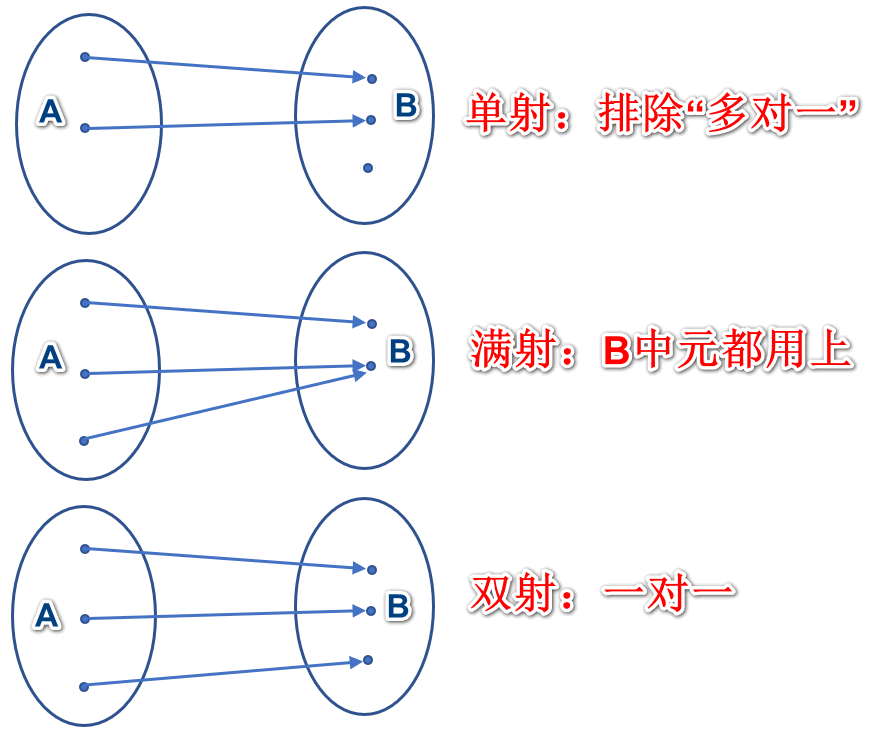
\includegraphics[width=0.5\textwidth]{image/mapping.png}
\caption{单射/满射/双射示意图} \label{fig:mapping}
\end{figure}

\begin{definition}
设~$f: \: A \rightarrow B$~为一一映射, 则对每个~$y \in B$, 都有唯一确定的~$x \in A$~满足~$y = f(x)$. 定义~$f^{-1}: \: B \rightarrow A$~为~$f^{-1}(y) = x$, 则称~$f^{-1}$~为~$f$~的逆映射.
\end{definition}

逆映射是反函数概念的推广, 由逆映射的定义
\[
f^{-1}\big(f(x)\big) = x, \quad x \in A
\]
\[
f\big(f^{-1}(y)\big) = y, \quad y \in B
\]

\begin{definition}
设映射~$f: \: A \rightarrow B, \, g: \: B \rightarrow C$, 定义~$g \circ f: \: A \rightarrow C$~为
\[
g \circ f(x) = g \big(f(x)\big), \quad x \in A
\]
称为~$f$~与~$g$~的复合映射.

设映射~$f: \: A \rightarrow B$, $A_0 \subset A$, 若~$g: \: A_0 \rightarrow B$~满足
\[
g(x) = f(x), \quad x \in A_0
\]
则称~$g$~为~$f$~在~$A_0$~上的限制, 记为~$g = f|_{A_0}$, 也称$f$~为~$g$~在~$A$~上的延拓.
\end{definition}

集合的特征函数是本书常用到的一种特殊映射. 

\begin{definition}
集合~$E$~的特征函数\index{特征函数}定义为
\[
\chi_E(x) = \left\{\!\!
\begin{array}{ll}
1, & x \in E \\
0, & x \notin E
\end{array}
\right.
\]
\end{definition}

特征函数~$\chi_E$~在一定意义上反映出集合~$E$~本身的特征, 可以通过它来表示各种集合关系. 例如, $A = B$~$\Leftrightarrow$~$\chi_A(x) = \chi_B(x)$; $A \subset B$~$\Leftrightarrow$~$\chi_A(x) \leqslant \chi_B(x)$. 容易验证:

(i) $\chi_{A \cap B}(x) = \chi_A(x) \cdot \chi_B(x)$;

(ii) $\chi_{A \cup B}(x) = \chi_A(x) + \chi_B(x) - \chi_A(x) \cdot \chi_B(x)$;

(iii) $\chi_{A - B}(x) = \chi_A(x) [1 - \chi_B(x)]$.

\begin{proposition}
对于映射, 下列事实成立:

(i) 若~$A \subset B$, 则~$f(A) \subset f(B)$;

(ii) $f\big(\smallcup\limits_{\alpha \in I} {A_\alpha} \big) = \smallcup\limits_{\alpha \in I} {f(A_\alpha)}$;

(iii) $f\big(\smallcap\limits_{\alpha \in I} {A_\alpha} \big) \subset \smallcap\limits_{\alpha \in I} {f(A_\alpha)}$, 当且仅当~$f$~为单射时, ``$=$''成立;

(iv) $f\big(f^{-1}(B)\big) \subset B$, 当且仅当~$f$~为满射时, ``$=$''成立;

 ~~~~~ $A \subset f^{-1}\big(f(A)\big)$, 当且仅当~$f$~为单射时, ``$=$''成立;

(v) $f^{-1}(B^c) = \big(f^{-1}(B)\big)^c$.
\end{proposition}

\begin{proof}
(i)~显然, (ii)~和~(v)~容易验证.

(iii) 只证明两个集合的情形. 注意到~$A_1 \cap A_2 \subset A_1, \, A_1 \cap A_2 \subset A_2$, 由~(i)~知
\[
f(A_1 \cap A_2) \subset f(A_1), \quad f(A_1 \cap A_2) \subset f(A_2)
\]
故~$f(A_1 \cap A_2) \subset f(A_1) \cap f(A_2)$.

设~$y \in f(A_1) \cap f(A_2)$, 则~$y \in f(A_1)$~且~$y \in f(A_2)$, 故存在~$x_1 \in A_1,\, x_2 \in A_2$~使得~$y = f(x_1) = f(x_2)$. 由于~$f$~是单射, 则必有~$x_1 = x_2 = x$. 所以
\[
x \in A_1 \cap A_2, \quad y = f(x) \in f(A_1 \cap A_2)
\]
故
\[
f(A_1) \cap f(A_2) \subset f(A_1 \cap A_2)
\]
因此, ``$=$''成立.

反之, 假设~$f$~不是单射, 则存在~$x_1 \neq x_2$~使得~$f(x_1) = f(x_2)$. 构造集合~$A_1 = \{x_1\}, \, A_2 = \{x_2\}$, 则~$A_1 \cap A_2 = \emptyset$, 从而~$f(A_1 \cap A_2) = \emptyset$. 而
\[
f(A_1) \cap f(A_2) = \{f(x_1)\} \neq \emptyset
\]
故~$f(A_1 \cap A_2) \neq f(A_1) \cap f(A_2)$. 矛盾.

(iv) (1) 设~$y \in f\big(f^{-1}(B)\big)$, 则存在~$x \in f^{-1}(B)$~使得~$y = f(x)$. 故~$y = f(x) \in B$. 因此, $f\big(f^{-1}(B)\big) \subset B$.

设~$y \in B$, $f$~为满射, 则存在~$x \in A$~使得~$y = f(x)$. 故~$x \in f^{-1}(y) \subset f^{-1}(B)$, 从而~$y = f(x) \in f\big(f^{-1}(B)\big)$, 于是~$B \subset f\big(f^{-1}(B)\big)$, 因此, ``$=$''成立.

反之, 假设~$f$~不是满射, 则~$f(A) \subsetneqq B$. 由于~$f^{-1}(B) \subset A$, 故
\[
f\big(f^{-1}(B)\big) \subset f(A) \subsetneqq B
\]
与~$B = f\big(f^{-1}(B)\big)$~矛盾.

(2) 设~$x \in A$, 则~$f(x) \in f(A)$, 故~$x \in f^{-1}\big(f(A)\big)$. 因此, $A \subset f^{-1}\big(f(A)\big)$.

设~$x \in f^{-1}\big(f(A)\big)$, 则~$f(x) \in f(A)$. 再由~$f$~是单射, 则必有~$x \in A$. 从而~$f^{-1}\big(f(A)\big) \subset A$. 因此, ``$=$''成立.

反之, 假设~$f$~不是单射, 则存在~$x_1 \neq x_2$~使得~$f(x_1) = f(x_2)$. 构造集合~$A = \{x_1\}$, 则~$f(A) = \{f(x_1)\}$. 故~$\{x_1, \, x_2\} \subset f^{-1}\big(f(A)\big)$, 从而~$A \neq f^{-1}\big(f(A)\big)$. 矛盾.
\end{proof}

\subsection{集合的对等}

研究集合的一个基本问题, 就是比较两个集合包含元素的多与少. 对于有限集, 我们可以通过分别数数的方法来比较. 例如, 比较某班学生人数与某教室座位数的多少, 就可以分别数出学生人数和座位个数, 然后比较两个数的大小来确定. 那么, 两个无限集是否可以比较元素的多少呢？

初看起来, 无限集都含有无限多个元素, 似乎不能比较元素的多与少, 现在我们换一种方式来考虑这个问题. 在比较两个有限集元素多少的时候, 还可以采用另一种方法, 即``一一对应''的方法. 比如前面的例子中, 可以考虑让一个学生坐一个座位(建立一一对应关系), 若学生和座位都恰好没有剩余, 则学生与座位数相等; 若仍有站着的学生, 则说明学生人数多; 若仍有空座位, 则说明座位数多.

用集合语言来描述就是, 若集~$A$~与~$B$~之间能建立一种一一对应, 则~$A$~与~$B$~具有同样多的元素. 如果~$A$~与~$B$~的一个真子集之间能建立一一对应, 则~$A$~的元素比~$B$~的元素少. 这种方法也适用于无限集的情形.

因此, 可以利用映射来研究比较两个集合元素多少的问题.

\begin{definition}
设~$A, \, B$~为非空集, 若存在从~$A$~到~$B$~的一一映射, 则称~$A$~与~$B$~对等\index{对等},
记为~$A \sim B$. 规定~$\emptyset \sim \emptyset$.
\end{definition}

$A$~与~$B$~对等就是两个集合的元素可以建立一一对应的关系. 对等关系具有如下性质:

(i) (反身性)$A \sim A$;

(ii) (对称性)若~$A \sim B$, 则~$B \sim A$;

(iii) (传递性)若~$A \sim B, \, B \sim C$, 则~$A \sim C$.

\medskip

\begin{example} \label{ex1.2.1}
自然数集~$\N$~$\sim$~正偶数集~$\sim$~正奇数集~$\sim$~整数集~$\Z$.
\end{example}

\begin{proof}
正偶数集~$= \{2n: \: n \in \N\}$; \quad 正奇数集~$= \{2n-1: \: n \in \N\}$;

\qquad \quad $\Z = \{(-1)^{n+1} [n/2]: \: n \in \N\}$.
\end{proof}

\medskip

\begin{example} \label{ex1.2.2}
$(-1, \, 1)~\sim~\R$.
\end{example}

\begin{proof}
$f(x) = \tan \dfrac{\pi}{2}x$.
\end{proof}

\medskip

\begin{example} \label{ex1.2.3}
\{去掉一点的圆周\}~$\sim~\R$.
\end{example}

\begin{proof}
如图~\ref{fig1.1.1}, 设圆周为~$C$, 从除去的点~$P$~作过圆心的直线, 取与该直线垂直且与圆周相切(不过点~$P$~)的直线
表示实轴~$\R$. 对于~$C - \{P\}$~上的每一点~$c$, 从点~$P$~作过点~$c$~的直线必与实轴相交于某点,
记为~$x$. 建立一一对应: $s: \: \R \rightarrow C - \{P\}$~为~$s(x) = c$. (点~$P$~对应~$\infty$)
\end{proof}

\begin{figure}[!htb]
\centering
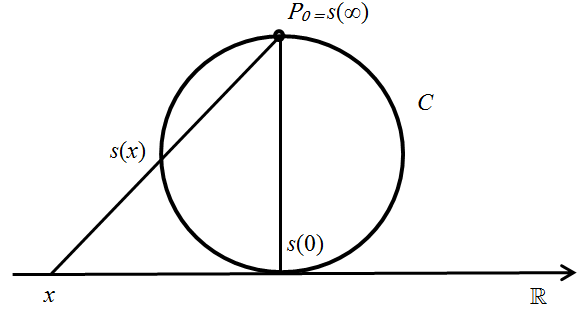
\includegraphics[width=0.56\textwidth]{image/duideng.png}
\caption{去掉一点的圆周与实轴对等} \label{fig1.1.1}
\end{figure}

类似地, 球面去掉一点与平面上的点集对等.

证明两个集合对等, 通常采用中间集合过渡(例~\ref{ex1.2.1})、寻找一一映射
(例~\ref{ex1.2.2})等方法. 另一个
重要方法就是利用伯恩斯坦定理.

\begin{lemma} \label{lem1.2.1}
设~$A,\,B$~为非空集, 若~$f: \: A \rightarrow B, \, g: \: B \rightarrow A$, 则~$A$~与~$B$~存在如下分解:

(i) $A = A_1 \cup A_2, \, B = B_1 \cup B_2$;

(ii) $A_1 \cap A_2 = \emptyset, \, B_1 \cap B_2 = \emptyset$;

(iii) $f(A_1) = B_1, \, g(B_2) = A_2$.
\end{lemma}

\begin{proof}
作集族
\[
\mathnormal{\Gamma} = \{E \subset A: \: E \cap g\big(B-f(E)\big) = \emptyset\}
\]
$\mathnormal{\Gamma}$~中的元称为~$A$~中的隔离集. 令~$A_1 = \smallcup \limits_{E \in \mathnormal{\Gamma}} E$, 则~$A_1 \in \mathnormal{\Gamma}$. 实际上, 对任意的~$E \in \mathnormal{\Gamma}$, 都有~$E \subset A_1$, 再由~$E \cap g\big(B-f(E)\big) = \emptyset$~知
\[
E \cap g\big(B-f(A_1)\big) = \emptyset
\]
从而
\[
A_1 \cap g\big(B-f(A_1)\big) = \smallcup \limits_{E \in \mathnormal{\Gamma}} \big[E \cap g\big(B-f(E)\big)\big] = \emptyset
\]
因此, $A_1$~是~$A$~中隔离集, 且是~$\mathnormal{\Gamma}$~中的最大元.

现在令~$B_1 = f(A_1), \, B_2 = B - B_1, \, A_2 = g(B_2)$, 则
\[
A_1 \cap A_2 = A_1 \cap g\big(B - f(A_1)\big) = \emptyset
\]
下面只需验证~$A_1 \cup A_2 = A$.

若不然, 则存在~$x_0 \in A, \, x_0 \notin A_1 \cup A_2$. 令~$A_0 = A_1 \cup \{x_0\}$, 由于~$B_1 = f(A_1) \subset f(A_0)$, 故
\[
B - f(A_0) \subset B - B_1 = B_2
\]
从而
\[
g\big(B - f(A_0)\big) \subset g(B_2) = A_2
\]
再由~$A_1 \cap A_2 = \emptyset$~以及~$x_0 \notin A_2$~知
\[
A_1 \cap g\big(B - f(A_0)\big) = \emptyset, \quad x_0 \notin g\big(B - f(A_0)\big)
\]
因此
\[
A_0 \cap g\big(B - f(A_0)\big) = \emptyset
\]
故~$A_0 \in \mathnormal{\Gamma}$. 这与~$A_1$~是~$\mathnormal{\Gamma}$~中的最大元矛盾.
\end{proof}

\begin{theorem}[伯恩斯坦定理\index{伯恩斯坦定理}] \label{Bernstein} 
若~$A$~与~$B$~的某子集对等, $B$~与~$A$~的某子集对等, 则~$A \sim B$.
\end{theorem}

\begin{proof}
由题设存在单射~$f: \: A \rightarrow B, \, g: \: B \rightarrow A$, 利用引理~\ref{lem1.2.1}~可得到~$A$~与~$B$~的分解
\[
A = A_1 \cup A_2, \quad B = B_1 \cup B_2
\]
\[
f(A_1) = B_1, \quad g(B_2) = A_2
\]
其中, $A_1 \cap A_2 = \emptyset, \, B_1 \cap B_2 = \emptyset$. 注意到~$f: \: A_1 \rightarrow B_1, \, g^{-1}: \: A_2 \rightarrow B_2$~是一一映射, 作映射
\[
F(x) = \left\{\!\!
\begin{array}{ll}
f(x), & x \in A_1 \\
g^{-1}(x), & x \in A_2
\end{array}
\right.
\]
则~$F: \: A \rightarrow B$~是一一映射, 从而~$A \sim B$.
\end{proof}

\medskip

\begin{example} \label{ex1.2.4}
$[-1,\,1] \sim \R$.
\end{example}

\begin{proof}
由例~\ref{ex1.2.2}, $\R \sim (-1,\,1) \subset [-1,\,1]$; 又~$[-1,\,1] \sim [-1,\,1] \subset \R$. 由伯恩斯坦定理, $[-1,\,1] \sim \R$.
\end{proof}

\subsection{集合的基数}

\begin{definition}
设~$A, \, B$~为两个集合, 若~$A \sim B$, 则称~$A$~与~$B$~的基数\index{基数}或势相同, 记为~$\overline{\overline A} = \overline{\overline B}$.
\end{definition}

由对等的传递性, 所有互相对等的集合都有相同的基数, 可见基数反映了对等集在元素数量级别上
的共性. 若~$A$~与
~$B$~的一个子集对等, 则~$\overline{\overline A} \leqslant \overline{\overline B}$. 结合映射的定义,  映射与基数之间存在如下关系:

(i) 若存在从~$A$~到~$B$~的单射, 则~$\overline{\overline A} \leqslant \overline{\overline B}$;

(ii) 若存在从~$A$~到~$B$~的满射, 则~$\overline{\overline A} \geqslant \overline{\overline B}$;

(iii) 若存在从~$A$~到~$B$~的一一映射, 则~$\overline{\overline A} = \overline{\overline B}$. \\
\noindent 因此, 伯恩斯坦定理也可以改写为下面的形式:

\begin{theorem}
若集合~$A,\,B$~满足~$\overline{\overline A} \leqslant \overline{\overline B}, \, \overline{\overline B} \leqslant \overline{\overline A}$, 则~$\overline{\overline A} = \overline{\overline B}$.
\end{theorem}

规定~$\overline{\overline{\emptyset}} = 0$. 若存在自然数~$n$, 使得~$A \sim \{1,\,2,\,\cdots, \, n\}$, 则称~$A$~为有限集, 并记~$\overline{\overline A} = n$. 因此有限集的基数等于该集合元素的个数. 这样,  集合的基数就是有限集元素个数的推广.

不是有限集的集合称为无限集. 有限集和无限集的本质区别在于: 有限集不能与其真子集对等,
而无限集必与其某个真子集对等.

\begin{theorem} \label{thm1.2.2}
有限集不可能与其某个真子集对等.
\end{theorem}

\begin{proof}
用数学归纳法证明, $n = 1$, 显然. 假设~$n = k$~时, 结论成立.

当~$n = k + 1$~时, 若存在~$A$~的某个真子集~$A_0$~使得~$A \sim A_0$, 则存在一一映射~$\varphi: \: A \rightarrow A_0$. 下面分两种情况:

(1) $\exists \, \ a \in A$, 使得~$\varphi(a) = a$.

令~$A_1 = A - \{a\}, \, A_2 = A_0 - \{a\}$, 则~$A_2$~是~$A_1$~的真子集, $\overline{\overline {A_1}} = k$. 而~$\varphi|_{A_1}$~是~$A_1$~到~$A_2$~的一一映射, 故~$A_1 \sim A_2$. 这与假设矛盾.

(2) $\forall \, a \in A$, 都有~$\varphi(a) \neq a$.

$A_0$~是~$A$~的真子集, 则存在~$x_0 \in A, \, x_0 \notin A_0$. 令
\[
A_3 = A - \{x_0\}, \quad A_4 = A_0 - \{\varphi(x_0)\}
\]
注意到~$x_0 \notin A_0$~以及~$A_0$~是~$A$~的真子集, 则~$A_4$~是~$A_3$~的子集. 又由于
\[
\varphi(x_0) \in A_0 \subset A, \quad \varphi(x_0) \neq x_0
\]
故~$\varphi(x_0) \in A - \{x_0\} = A_3$, 而~$\varphi(x_0) \notin A_0 - \{\varphi(x_0)\} = A_4$. 从而~$A_4$~是~$A_3$~的真子集,  于是~$\overline{\overline {A_3}} = k$, ~$\varphi|_{A_3}$~是~$A_3$~到~$A_4$~的一一映射, 故~$A_3 \sim A_4$. 这与假设矛盾.
\end{proof}

\section{可列集}

\subsection{可列集的定义}

无限集中最简单、最常见、包含元素个数最少的一类就是可列集.

\begin{definition}
与自然数集~$\N$~对等的集合称为可列集\index{可列集},
其基数记为~$\aleph_0$(读作阿列夫零). 有限集和可列集统称
为可数集\index{可数集}.
\end{definition}

\begin{remark}
$A$~是可列集, 当且仅当~$A$~可以写成~$A = \{a_n\}_{n = 1} ^\infty$.
\end{remark}

\begin{proof}
$A$~可列, 则存在~$\N$~到~$A$~的一一映射~$\varphi$, 记为~$\varphi(n) = a_n, \, n \in \N$, 则~$A = \{a_n\}_{n = 1} ^\infty$. 反过来, 若~$A = \{a_n\}_{n = 1} ^\infty$, 将每个~$a_n$~与其下标~$n$~建立一一对应, 则~$A$~与~$\N$~对等, 从而是可列集.
\end{proof}

由~\S~1.2~例~\ref{ex1.2.1}, 自然数集、正偶数集、正奇数集、整数集都是可列集.

\subsection{可列集的性质}

\begin{proposition} \label{thm1.3.1}
任何无限集必包含一个可列子集.
\end{proposition}

\begin{proof}
设~$A$~为无限集. 从~$A$~中任取一元~$a_1$; 由于~$A - \{a_1\} \neq \emptyset$, 取~$a_2 \in A - \{a_1\}$; 又~$A - \{a_1, \, a_2\} \neq \emptyset$, 取~$a_3 \in A - \{a_1, \, a_2\}$; $\cdots\cdots$,  因为~$A$~是无限集, 这一过程可以一直继续下去, 从而得到~$A$~的一个可列子集~$\{a_n\}_{n = 1} ^\infty$.
\end{proof}

该定理也说明, 众多无限集中, 最小的基数是可列集的基数~$\aleph_0$.

\begin{corollary} \label{cor1.3.1}
无限集必与其某个真子集对等.
\end{corollary}

\begin{proof}
设~$A$~为无限集, 由定理~\ref{thm1.3.1}, 存在可列子集~$\{a_n\}_{n = 1} ^\infty \subset A$. 令~$B = A - \{a_1\}$, 则~$B$~是~$A$~的真子集. 定义映射
\begin{eqnarray*}
\varphi(a_k) &=& a_{k+1}, \quad k = 1, \, 2, \, \cdots \\
\varphi(x) &=& x, \quad x \in A - \{a_n\}_{n = 1} ^\infty
\end{eqnarray*}
则~$\varphi: \: A \rightarrow B$~是一一映射, 故~$A \sim B$.
\end{proof}

结合定理~\ref{thm1.2.2}~与推论~\ref{cor1.3.1}, 可以得到有限集和无限集的如下等价定义
\[
\left\{\!\!
\begin{array}{lcl}
A \mbox{~是有限集~} & \Longleftrightarrow & A \mbox{~不与其任意真子集对等~} \\
A \mbox{~是无限集~} & \Longleftrightarrow & A \mbox{~必与其某个真子集对等~}
\end{array}
\right.
\]

\begin{proposition} \label{thm1.3.2}
可列集的任何无限子集都是可列集.
\end{proposition}

\begin{proof}
设~$A = \{a_1, \, a_2, \, \cdots, \, a_n, \, \cdots\}$. $B$~是~$A$~的无限子集, 按照~$A$~中元素的次序依次寻找~$B$~中元素, 分别记为~$a_{n_1},\, a_{n_2}, \, \cdots$, 则~$B = \{a_{n_1}, \, a_{n_2}, \, \cdots, \, a_{n_k}, \, \cdots\}$~为可列集.
\end{proof}

\begin{proposition} \label{thm1.3.4}
有限集与可列集的并集是可列集.
\end{proposition}

\begin{proof}
设~$A = \{a_1, \, a_2, \, \cdots, \, a_n\}, \, B = \{b_1, \, b_2, \, \cdots\}$. 不妨设~$A \cap B = \emptyset$, 则
\[
A \cup B = \{a_1, \, a_2, \, \cdots, \, a_n, \, b_1, \, b_2, \, \cdots\}
\]
可列.
\end{proof}

\begin{proposition} \label{thm1.3.5}
有限个可列集的并集是可列集.
\end{proposition}

\begin{proof}
设~$A_k = \{a_1 ^{(k)}, \, a_2 ^{(k)}, \, a_3 ^{(k)}, \, \cdots\}, \, k = 1,\,2,\, \cdots, \,n$~为可列集, 则~$\smallcup \limits_{k=1} ^n A_k$~的元素可以按下面的方式编号排序
\[
\begin{array}{cccccc}
A_1 & = & \{~a_1 ^{(1)} & a_2 ^{(1)} & a_3 ^{(1)} & \cdots~\} \\
    &   &   \downarrow  & \downarrow & \downarrow &           \\
A_2 & = & \{~a_1 ^{(2)} & a_2 ^{(2)} & a_3 ^{(2)} & \cdots~\} \\
    &   &   \downarrow  & \downarrow & \downarrow &           \\
    &   &   \vdots      &    \vdots  &    \vdots  &           \\
    &   &   \downarrow  & \downarrow & \downarrow &           \\
A_n & = & \{~a_1 ^{(n)} & a_2 ^{(n)} & a_3 ^{(n)} & \cdots~\}
\end{array}
\]
必要时删掉后续的重复元, 可得到
\[
\medcup \limits_{k=1} ^n A_k = \big\{a_1 ^{(1)}, \, \cdots, \, a_1 ^{(n)}, \, a_2 ^{(1)}, \, \cdots, \, a_2 ^{(n)}, \, a_3 ^{(1)}, \, \cdots\big\}
\]
可列.
\end{proof}

\begin{proposition} \label{thm1.3.6}
可列个可列集的并集是可列集.
\end{proposition}

\begin{proof}
设~$\{A_n\}_{n=1} ^\infty$~为一列可列集, 则~$\smallcup \limits_{n=1} ^\infty A_n$~的元素可以按下面的方式编号排序
\[
\begin{array}{cccccccccc}
A_1 &=& \{~a_1 ^{(1)} & \rightarrow & a_2 ^{(1)} && a_3 ^{(1)} & \rightarrow & a_4 ^{(1)} & \cdots~\} \\
    &&                &  \swarrow   &      & \nearrow &        &  \swarrow   &            &   \\
A_2 &=& \{~a_1 ^{(2)} &  & a_2 ^{(2)} && a_3 ^{(2)} &  & a_4 ^{(2)} & \cdots~\} \\
    &&   \downarrow   &  \nearrow   &      & \swarrow &        &  &  &   \\
A_3 &=& \{~a_1 ^{(3)} &  & a_2 ^{(3)} && a_3 ^{(3)} &  & a_4 ^{(3)} & \cdots~\} \\
    & &     \vdots    &  &   \vdots   &&    \vdots  &  &   \vdots   &           \\
A_n &=& \{~a_1 ^{(n)} &  & a_2 ^{(n)} && a_3 ^{(n)} &  & a_4 ^{(n)} & \cdots~\} \\
    & &     \vdots    &  &    \vdots  &&    \vdots  &  &   \vdots   &
\end{array}
\]
必要时删掉后续的重复元, 可得到
\[
\medcup \limits_{n=1} ^\infty A_n = \big\{a_1 ^{(1)}, \, a_2 ^{(1)}, \, a_1 ^{(2)}, \, \cdots, \, a_1 ^{(2n+1)}, \, a_2 ^{(2n)}, \, \cdots, \, a_{2n+1} ^{(1)}, \, \cdots\big\}
\]
(依次是下标之和等于~$2, \, 3, \, \cdots, \, 2n+2, \, \cdots$)可列.
\end{proof}

\begin{proposition} \label{thm1.3.7}
若~$A$~为无限集, $B$~为有限集或可列集, 则~$\overline{\overline{A \cup B}} = \overline{\overline{A}}$.
\end{proposition}

\begin{proof}
不妨设~$A \cap B = \emptyset$, 否则用~$B - A$~代替~$B$~即可. $A$~为无限集, 由定理~\ref{thm1.3.1}, $A$~包含一个可列子集~$A_1$. 由于~$A_1 \cup B$~是可列集, 故~$A_1 \cup B \sim A_1$. 注意到~$(A - A_1) \cap (A_1 \cup B) = \emptyset$, 则有
\begin{eqnarray*}
A \cup B &=& (A - A_1) \cup A_1 \cup B \\
&=& (A - A_1) \cup (A_1 \cup B) \sim (A - A_1) \cup A_1 = A
\end{eqnarray*}
因此, $\overline{\overline{A \cup B}} = \overline{\overline{A}}$.
\end{proof}

\subsection{可列集的例}

\begin{example} \label{ex1.3.1}
有理数集~$\Q$~是可列集.
\end{example}

\begin{proof}
$\Q = \Q^+ \cup \{0\} \cup \Q^-$, 其中~$\Q^+, \, \Q^-$~分别表示正、负有理数集. 由对称性以及定理~\ref{thm1.3.4}~和
定理~\ref{thm1.3.5}, 只需证明$\Q^+$~可列.

对每个~$n \in \N$, 令
\[
A_n = \Big\{\frac{1}{n},\,\frac{2}{n},\,\frac{3}{n},\,\cdots\Big\}
\]
则~$A_n$~可列. 又~$\Q^+ = \smallcup \limits_{n=1} ^\infty A_n$(除去重复元), 由可列集性质知~$\Q^+$~可列.
\end{proof}

\medskip

\begin{example} \label{ex1.3.2}
实轴上互不相交的开区间至多有可列个.
\end{example}

\begin{proof}
开区间的长度大于~$0$, 故必含有有理数, 在每一个开区间内取出一个有理数. 因为开区间互不相交,
所以取出的有理数都不相等, 从而这些有理数构成~$\Q$~的一个子集. 又~$\Q$~是可列集,
故这样的开区间至多有可列个.
\end{proof}

\medskip

\begin{example} \label{ex1.3.3}
设~$A, \, B$~为可列集, 则~$A \times B$~是可列集.
\end{example}

\begin{proof}
注意到
\[
A \times B = \big\{(x,\,y): \: x \in A, \, y \in B\big\} = \medcup_{x \in A} \big\{(x,\,y): \: y \in B\big\}
\]
由可列集性质知~$A \times B$~可列.
\end{proof}

\begin{remark} \label{rem1.3.2}
类似地, 用数学归纳法易证: 若~$A_1,\, A_2,\, \cdots,\, A_n$~可列, 则
\[
A_1 \times A_2 \times \cdots \times A_n
\]
可列.
\end{remark}

\medskip

\begin{example} \label{ex1.3.4}
整系数多项式的全体~$\mathbf{P}$~是可列集.
\end{example}

\begin{proof}
对每个~$n \in \{0\} \cup \N$, 令
\[
P_n = \big\{a_0 x^n + a_1 x^{n-1} + \cdots + a_n: \: a_i \in \Z, \, i=0,\,1,\, \cdots, \,n, \, a_0 \neq 0\big\}
\]
则
\[
P_n \sim \Z-\{0\} \times \overbrace{\Z \times \cdots \times \Z}^{\tiny n\mbox{\tiny 个}}
\]
由注~\ref{rem1.3.2}~知~$P_n$~可列. 又~$\mathbf{P} = \mathop{\cup} \limits_{n = 0} ^\infty P_n$, 由可列集性质知~$\mathbf{P}$~可列.
\end{proof}

整系数多项式的根称为代数数, 由于每个多项式只有有限个根, 故代数数的全体构成一可列集.

\medskip

\begin{example} \label{ex1.3.5}
$\R$~上单调函数的不连续点至多有可列个.
\end{example}

\begin{proof}
不妨设~$f$~单调递增, 若~$x_0$~是~$f$~的不连续点, 则
\[
f(x_0 - 0) = \lim_{x \to x_0 ^-} f(x) < \lim_{x \to x_0 ^+} f(x) = f(x_0 + 0)
\]
故~$x_0$~就对应着一个开区间~$\big( f(x_0 - 0), \, f(x_0 + 0) \big)$. 显然, 若~$x_1, \, x_2$~是~$f$~的不同不连续点, 则对应区间~$\big( f(x_1 - 0), \, f(x_1 + 0) \big)$~与~$\big( f(x_2 - 0), \, f(x_2 + 0) \big)$~互不相交. 而~$\R$~上互不相交的开区间至多有可列个,
故~$f$~的不连续点也至多有可列个.
\end{proof}

\subsection{不可列集, 连续基数}

下面的定理表明不可列集是存在的.

\begin{theorem}
$[0,1]$~是不可列集.
\end{theorem}

\begin{proof}
假设~$[0,1]$~可列, 则可表示为~$[0,1] = \{x_n\}_{n=1}^\infty$.

把~$[0,1]$~三等分为: $[0,\,1/3], \, [1/3,\,2/3], \, \big[2/3,\,1]$, 则其中至少有一个闭区间不包含~$x_1$, 记该区间为~$I_1$, 则~$x_1 \notin I_1$; 把~$I_1$~三等分, 则其中至少有一个闭区间不包含~$x_2$, 记该区间为~$I_2$, 则~$x_2 \notin I_2, \, I_2 \subset I_1$; $\cdots\cdots$, 依次做下去, 可得到一列闭区间~$\{I_n\}$~满足:

(i) $I_1 \supset I_2 \supset \cdots \supset I_n \supset \cdots$;

(ii) $x_n \notin I_n, \, n \in \N$;

(iii) $I_n$~的长度为~$1/3^n \rightarrow 0, \, n \rightarrow \infty$.

由闭区间套定理, 存在~$\xi \in \mathop{\cap} \limits_{n=1} ^\infty I_n$. 由于~$\xi \in [0,1] = \{x_n\}_{n=1}^\infty$, 则必存在~$n_0 \in \N$~使得~$\xi = x_{n_0}$. 而~$x_{n_0} \notin I_{n_0}$, 这与~$\xi \in \mathop{\cap} \limits_{n=1} ^\infty I_n$~矛盾.
\end{proof}

\begin{definition}
若~$A \sim [0,1]$, 则称~$A$~具有连续基数\index{连续基数}, 记~$\overline{\overline{A}} = \aleph$.
\end{definition}

\begin{theorem}
$\overline{\overline{[a,\,b]}} = \overline{\overline{(a,\,b)}} = \overline{\overline{(a,\,b]}} = \overline{\overline{\R}} = \aleph$.
\end{theorem}

\begin{proof}
映射~$f(x) = a + (b - a)x$~建立了~$[0,\,1]$~与~$[a,\,b]$~之间的一一对应, 故~$\overline{\overline{[a,\,b]}} = \aleph$. 又~$(a,\,b)$~和~~$(a,\,b]$~与~$[a,\,b]$~分别只差一个点和两个点, 由定理~\ref{thm1.3.7}~知~$
\overline{\overline{(a,\,b)}} = \overline{\overline{(a,\,b]}} = \overline{\overline{[a,\,b]}} = \aleph$.
最后, 由~\S~1.2~例~\ref{ex1.2.4}~以及前面的结论可得, $\overline{\overline{\R}} = \overline{\overline{[-1,\,1]}} = \aleph$.
\end{proof}

\begin{corollary}
无理数的基数为~$\aleph$.
\end{corollary}

\begin{proof}
记无理数集为~$\mathbb{I}$, 注意到~$\mathbb{I} \cup \Q = \R$, 且~$\Q$~可列, 由定理~\ref{thm1.3.7}~可得~$\overline{\overline{\mathbb{I}}} = \overline{\overline{\mathbb{I} \cup \Q}} = \overline{\overline{\R}} = \aleph$.
\end{proof}

\begin{theorem}
设~$\{A_n\}$~为一集列, 若对每个~$n$~都有~$\overline{\overline{A_n}} = \aleph$, 则~$\overline{\overline{\mathop{\cup}\limits_{n=1}^\infty A_n}} = \aleph$.
\end{theorem}

\begin{proof}
不妨设~$A_i \cap A_j = \emptyset$. 由于~$\overline{\overline{A_n}} = \aleph$, 则~$A_n \sim (n,\,n+1]$, 从而~$\smallcup\limits_{n=1}^\infty A_n \sim [1,\,\infty) \sim \R$.
\end{proof}

设~$A$~为集合, 记~$2^A$~为~$A$~的幂集. 若~$A$~为~含有~$n$~个元素的有限集, 则~$2^A$~由~$1$~个空集,
$\mathrm{C}_n ^1$~个单元素集, $\mathrm{C}_n ^2$~个两元素集, $\cdots\cdots,\, \mathrm{C}_n^n$~个~$n$~元素集,  所以, $2^A$~中元素的个数为
\[
1 + \mathrm{C}_n ^1 + \mathrm{C}_n ^2 + \cdots + \mathrm{C}_n ^n = (1 + 1)^n = 2^n = 2^{\overline{\overline{A}}}
\]
更一般地, 设~$\overline{\overline{A}} = \mu$, 定义~$\overline{\overline{2^A}} = 2^\mu$.

对于每个~$E \in 2^A$, 可以唯一的对应一个特征函数
\[
\chi_E(x) = \left\{\!\!
\begin{array}{ll}
1, & x \in E \\
0, & x \in A - E
\end{array}
\right.
\]
反之亦然. 这说明~$A$~上所有特征函数的全体与~$2^A$~对等.

\begin{theorem} \label{thm1.3.11}
$\aleph = 2^{\aleph_0}$.
\end{theorem}

\begin{proof}
用~$\mathcal{F_{\N}}$~表示~$\N$~上特征函数的全体, 只需证
~$\mathcal{F_{\N}}$~与~$(0,\,1]$~对等.

对任意的~$\varphi \in \mathcal{F_{\N}}$, 作映射
\[
f: \: \varphi \rightarrow \sum_{n=1} ^\infty \frac{\varphi(n)}{3^n}
\]
易知, $f$~是从~$\mathcal{F_{\N}}$~到~$(0,\,1]$~的单射, 故
~$\overline{\overline{\mathcal{F_{\N}}}} \leqslant \overline{\overline{(0,\,1]}}$.

另一方面, 对每一个~$x \in (0,\,1]$, 用~$2$~进制表示为(不进位)
\[
x = \sum_{n=1} ^\infty \frac{a_n}{2^n}, \quad a_n \in \{0,\,1\}
\]
定义映射
\[
g: \: x \rightarrow \varphi \in \mathcal{F_{\N}}, \quad \varphi(n) = a_n, \quad n = 1, \,2, \, \cdots
\]
易知, $g$~是从~$(0,\,1]$~到~$\mathcal{F_{\N}}$~的单射, 故
~$\overline{\overline{(0,\,1]}} \leqslant \overline{\overline{\mathcal{F_{\N}}}}$.

由伯恩斯坦定理, $\overline{\overline{(0,\,1]}} = \overline{\overline{\mathcal{F_{\N}}}}$.
\end{proof}

\medskip

\begin{example}
$\R^2 \sim \R$.
\end{example}

\begin{proof}
由于~$\R \sim 2^{\N} \sim 2^{\Z - \N}$, 故~$\R \times \R \sim 2^{\N} \times 2^{\Z - \N} \sim 2^{\Z} \sim 2^{\N} \sim \R$.
\end{proof}

\medskip

\begin{example}
用~$M$~表示~$[0,\,1]$~上实值有界函数的全体, 则~$\overline{\overline{M}} = 2^\aleph$.
\end{example}

\begin{proof}
设~$E$~为~$[0,\,1]$~的任一子集, 则~$E$~唯一对应一个特征函数
\[
\chi_E(x) = \left\{\!\!
\begin{array}{ll}
1, & x \in E \\
0, & x \in [0,\,1] - E
\end{array}
\right.
\]
显然, $\chi_E \in M$. 故~$\overline{\overline{M}} \geqslant \overline{\overline{2^{[0,1]}}} = 2^\aleph$.

另一方面, 对每一个~$f \in M$, 其图像~$\{\big(x,\,f(x)\big): \: x \in [0,\,1]\}$~为平面上的一有界子集,
两者构成一一对应关系, 故~$\overline{\overline{M}} \leqslant \overline{\overline{2^{\R^2}}} = \overline{\overline{2^\R}} = 2^\aleph$. 由伯恩斯坦定理, $\overline{\overline{M}} = 2^\aleph$.
\end{proof}

\begin{theorem}[无最大基数定理\index{无最大基数定理}]
设~$A$~为非空集, 则~$\overline{\overline{A}} < \overline{\overline{2^A}}$.
\end{theorem}

\begin{proof}
由于~$2^A$~中的单元素集与~$A$~对等, 故~$\overline{\overline{A}} \leqslant \overline{\overline{2^A}}$.

若存在集合~$A$~满足~$\overline{\overline{A}} = \overline{\overline{2^A}}$, 则存在~$f: \: A \rightarrow 2^A$~为一一映射. 令
\[
B = \{x \in A: \: x \notin f(x)\}
\]
注意到~$\emptyset \in 2^A$, 则存在~$x_0 \in A$~使得~$f(x_0) = \emptyset$, 故~$x_0 \notin f(x_0)$. 这说明~$x_0 \in B$, 从而~$B \neq \emptyset$.

又~$B \in 2^A$, 则存在~$x_B \in A$~使得~$f(x_B) = B$. 下面考察~$x_B$~与~$B$~的关系: 若~$x_B \in B$, 则~$x_B \notin f(x_B) = B$, 矛盾; 若~$x_B \notin B$, 即~$x_B \notin f(x_B)$, 这又蕴涵~$x_B \in B$, 矛盾.
\end{proof}



\section{$\R^n$~中开集、闭集及其性质}

本节将讨论~$\R^n$~中的一些常见的点集及其拓扑性质.

\subsection{$n$~维欧氏空间}

我们用~$\R^n$~表示~$n$~维欧氏空间\index{欧氏空间}, 即
\[
\R^n = \big\{(x_1,\,x_2,\, \cdots, \, x_n): \: x_1,\,x_2,\, \cdots, \, x_n \in \R\big\}
\]
其中, $x_i$~称为~$x$~的第~$i$~个坐标.

设~$x = (x_1,\,x_2,\, \cdots, \, x_n), \, y = (y_1,\,y_2,\, \cdots, \, y_n) \in \R^n, \, k \in \R$, 按如下的加法、数乘
\[
x + y = (x_1 + y_1,\, x_2 + y_2, \, \cdots, \, x_n + y_n)
\]
\[
k x = (k x_1,\, k x_2, \, \cdots, \, k x_n)
\]
构成线性空间.

对于任意的~$x,\,y \in \R^n$, 定义
\[
d(x,\,y) = \Big( \sum_{i=1} ^n |x_i - y_i|^2 \Big)^\frac{1}{2}
\]
表示点~$x$~到~$y$~的距离. 容易验证, 距离满足下列性质:

(i) (非负性) $d(x,\,y) \geqslant 0$, $d(x,\,y) = 0$~当且仅当~$x = y$;

(ii) (对称性) $d(x,\,y) = d(y,\,x)$;

(iii) (三角不等式) 对任意的~$x,\,y,\,z \in \R^n$, 都有
\[
d(x,\,y) \leqslant d(x,\,z) + d(z,\,y)
\]

通常记~$d(x,\,0) = \|x\|$, 表示~$x$~的范数, 若~$x \in \R^1$, 则~$\|x\|$~即为~$x$~的绝对值.

\begin{definition}
设~$\{x_k\}$~为~$\R^n$~中的点列, 若存在~$x \in \R^n$~使得
\[
\lim_{k \to \infty} d(x_k, \, x) = 0
\]
则称~$\{x_k\}$~收敛于~$x$, 记为~$\lim\limits_{k \to \infty} x_k = x$~或~$x_k \rightarrow x(k \to \infty)$.
\end{definition}

设~$x_k = \big(\xi_1 ^{(k)}, \, \xi_2 ^{(k)}, \, \cdots, \, \xi_n ^{(k)}\big), \, x = (\xi_1,\,\xi_2,\, \cdots, \, \xi_n)$. 注意到
\[
|\xi_i ^{(k)} - \xi_i| \leqslant d(x_k,\,x) \leqslant \sum_{i = 1}^n |\xi_i ^{(k)} - \xi_i|
\]
易证~$x_k \rightarrow x$, 当且仅当对每个坐标位置~$i$, 都有~$\xi_i ^{(k)} \rightarrow \xi_i(k \to \infty)$. 再由柯西收敛准则可得:

\begin{proposition}
设~$\{x_k\} \subset \R^n$, 则~$\{x_k\}$~是收敛列, 当且仅当
\[
\lim_{i,j \to \infty} d(x_i,\,x_j) = 0
\]
\end{proposition}

\subsection{$\R^n$~中的开集及其性质}

\begin{definition}
设~$x_0 \in \R^n, \, \varepsilon > 0$, 定义
\[
U(x_0,\,\varepsilon) = \{x \in \R^n: \: d(x,\, x_0) < \varepsilon\}
\]
为~$x_0$~的~$\varepsilon-$邻域\index{邻域}.

设~$A \subset \R^n, \, x \in A$, 若存在~$\varepsilon_0 > 0$~使得~$U(x,\,\varepsilon_0) \subset A$, 则称~$x$~为~$A$~的内点. $A$~的全体内点, 记为~$A^\circ$.

若~$A$~中每个点都是~$A$~的内点\index{内点}, 则称~$A$~为开集\index{开集}.
\end{definition}

例如, $(a, \, b), \, (-\infty, \, a), \, (a, \, +\infty)$~都是~$\R$~中的开集; 邻域~$U(x_0,\,r)$, 又称以~$x_0$~为心、以~$r$~为半径的开球, 是~$\R^n$~中的开集; $A^\circ$~也是开集.

\begin{proposition} \label{prop1.4.2}
开集具有以下性质:


(i) $\emptyset$~和~$\R^n$~是开集;

(ii) 任意个开集的并集是开集;

(iii) 有限个开集的交集是开集.
\end{proposition}

\begin{proof}
(i) 显然.

(ii) 设~$\{G_\alpha: \: \alpha \in \mathnormal{\Gamma}\}$~为一族开集. 任取~$x \in \smallcup\limits_{\alpha \in \mathnormal{\Gamma}} G_\alpha$, 则存在~$\alpha_0 \in \mathnormal{\Gamma}$~使得~$x \in G_{\alpha_0}$.  由于~$G_{\alpha_0}$~是开集, 则存在~
$\varepsilon_0 > 0$~使得
\[
U(x,\,\varepsilon_0) \subset G_{\alpha_0} \subset \medcup_{\alpha \in \mathnormal{\Gamma}} G_\alpha
\]
故~$x$~是~$\smallcup\limits_{\alpha \in \mathnormal{\Gamma}} G_\alpha$~的内点.  再由~$x$~的任意性知~$\smallcup\limits_{\alpha \in \mathnormal{\Gamma}} G_\alpha$~是开集.

(iii) 设~$G_1,\,G_2,\,\cdots,\,G_n$~为开集, 任取~$x \in \smallcap\limits_{i=1}^n G_i$,
则~$x \in G_i,\, i=1,\,2,\,\cdots,\,n$. 由于~$G_i$~是开集, 故存在~$\varepsilon_i > 0$~使得
\[
U(x,\,\varepsilon_i) \subset G_i, \quad i = 1,\,2,\,\cdots,\,n
\]
令~$\varepsilon = \min\{\varepsilon_1,\,\varepsilon_2,\,\cdots,\,\varepsilon_n\}$, 则~$\varepsilon > 0$~且~$U(x,\,\varepsilon) \subset \smallcap\limits_{i=1}^n G_i$,\  故~$x$~是~$\smallcap\limits_{i=1}^n G_i$~的内点. 再由~$x$~的任意性知
~$\smallcap\limits_{i=1}^n G_i$~是开集.
\end{proof}

\begin{remark}
无限个开集的交集不一定是开集. 例如
\[
\medcap\limits_{n=1}^\infty \Big(-\frac{1}{n},\,\frac{1}{n}\Big) = \big\{0\big\}
\]
\end{remark}

\begin{theorem}
$A^\circ$~为开集.
\end{theorem}

\begin{proof}
任取~$x \in A^\circ$, 则存在~$r > 0$~使得~$U(x,\,r) \subset A$. 对~$\forall~y \in U(x,\,r)$, 令~$\delta = r - d(x,\,y)$, 则易知~$U(y,\,\delta) \subset A$, 故~$y \in A^\circ$. 从而~$U(x,\,r) \subset A^\circ$, 因此, $A^\circ$~是开集.
\end{proof}

\subsection{$\R^n$~中的闭集及其性质}

\begin{definition}
设~$x_0 \in \R^n, \, A \subset \R^n$. 若对~$\forall~\varepsilon > 0$, 都有
\[
U(x_0,\,\varepsilon) \cap \big(A - \{x_0\}\big) \neq \emptyset
\]
则称~$x_0$~为~$A$~的聚点\index{聚点}或极限点.
\end{definition}

\begin{remark}
(i) 聚点不一定属于~$A$. 例如, $A = (0,\,1)$, $[0,\,1]$~都是~$A$~的聚点.

(ii) 若~$x_0$~是~$A$~的聚点, 则对~$\forall~\varepsilon > 0$, $U(x,\,\varepsilon)$~中含有无穷多~$A$~中的点.

\begin{proof}
假设存在~$\varepsilon_0 > 0$, 使得
\[
U(x_0,\,\varepsilon_0) \cap \big(A - \{x_0\}\big) = \{x_1,\,x_2,\,\cdots,\,x_n\}
\]
令
\[
\delta = \min\{|x_0 - x_i|: \: i=1,\,2,\, \cdots, \, n\}
\]
则~$U(x_0,\,\delta)$~中不含~$A$~中异于~$x_0$~的点, 这与~$x_0$~是~$A$~的聚点矛盾.
\end{proof}
\end{remark}

\begin{definition}
设~$A \subset \R^n$, 则~$A$~的聚点的全体, 称为~$A$~的导集, 记为~$A'$. 若~$A' = A$, 则称~$A$~为完全集(无孤立点).

$A - A'$~中的点, 称为孤立点.

$A \cup A'$~称为~$A$~的闭包, 记为~$\overline{A}$.

开集的余集, 称为闭集\index{闭集}.
\end{definition}

例如, $[a, \, b], \, (-\infty, \, a], \, [a, \, +\infty)$~都是~$\R$~中的闭集; 以~$x_0$~为心, 以~$r$~为半径的闭球~$B(x_0,\,r) = \{x \in \R^n: \: d(x,\,x_0) \leqslant r\}$~是~$\R^n$~中的闭集; $A',\,\overline{A}$~也是闭集.

\begin{proposition}
利用导集的定义容易验证:

(i) 若~$A \subset B$, 则~$A' \subset B'$;

(ii) $(A \cup B)' = A' \cup B'$.
\end{proposition}

由命题~\ref{prop1.4.2}, 闭集的定义以及德·摩根公式, 容易得到下面的命题:

\begin{proposition}
闭集具有以下性质:

(i) $\emptyset$~和~$\R^n$~是闭集;

(ii) 任意个闭集的交集是闭集;

(iii) 有限个闭集的并集是闭集.
\end{proposition}

\begin{remark}
无限个闭集的并集不一定是闭集. 例如, $\smallcup\limits_{n=1}^\infty \big[1/n,\,1\big] = (0,\,1]$.
\end{remark}

\begin{proposition} \label{prop1.4.5}
设~$A \subset \R^n$, 则:
(i) $x \in A'~\Leftrightarrow~\exists~\{x_n\} \subset \big(A - \{x\}\big)$~使得~$x_n \rightarrow x$;

(ii) $x \in \overline{A}~\Leftrightarrow~\exists~\{x_n\} \subset A$~使得~$x_n \rightarrow x$.
\end{proposition}

\begin{proof}
(i) ``$\Rightarrow$''. 若~$x \in A'$, 则对~$\forall~\varepsilon > 0$, 都有~$U(x,\,\varepsilon) \cap \big(A - \{x\}\big) \neq \emptyset$. 特别地, 依次令~$\varepsilon_n = 1/n, \, n =1,\,2,\,\cdots$, 取~$x_n \in U\big(x,\,1/n\big) \cap \big(A - \{x_0\}\big)$, 则~$x_n \rightarrow x$.

``$\Leftarrow$''. 设~$\{x_n\} \subset \big(A - \{x\}\big)$~满足~$x_n \rightarrow x$. 由于~$x_n \rightarrow x$, 则对~$\forall~\varepsilon > 0$, $\exists~N \in \N$, 使得当~$n \geqslant N$~时有~$d(x_n,\,x) < \varepsilon$, 即~$x_n \in U(x,\,\varepsilon), \, \forall~n \geqslant N$. 又~$x_n \neq x$, 故~$U(x,\,\varepsilon) \cap \big(A - \{x\}\big) \neq \emptyset$. 因此, $x \in A'$.

(ii) ``$\Rightarrow$''. $\overline{A} = A \cup A'$. 若~$x \in A$, 令~$x_n = x, \, n \in \N$, 则~$x_n \rightarrow x$. 若~$x \in A'$, 由~(i)~知, 结论仍然成立.


``$\Leftarrow$''. 设~$\{x_n\} \subset A$~满足~$x_n \rightarrow x$. 若~$\exists~n_0 \in \N$, 使得~$x_{n_0} = x$, 则~$x \in A \subset \overline{A}$. 否则~$\forall~n \in \N$, 都有~$x_n \neq x$, 则由~(i)~知, $x \in A' \subset \overline{A}$.
\end{proof}

\begin{theorem} \label{thm1.4.3}
$A$~为闭集~$\Leftrightarrow$~$A' \subset A$.
\end{theorem}

\begin{proof}
``$\Rightarrow$''. 设~$A$~为闭集, 则~$A^c$~为开集. 任取~$x \in A'$, 往证~$x \in A$, 即~$x \notin A^c$. 若~$x \in A^c$, 由于~$A^c$~是开集, 则存在~$\varepsilon_0 > 0$~使得~$U(x,\,\varepsilon_0) \subset A^c$. 故~$U(x,\,\varepsilon_0) \cap A = \emptyset$, 从而~$U(x,\,\varepsilon_0) \cap \big(A - \{x\}\big) = \emptyset$. 这与~$x \in A'$~矛盾.

``$\Leftarrow$''. 设~$A' \subset A$, 往证~$A$~是闭集, 即~$A^c$~是开集. 任取~$x \in A^c$, 由于~$A' \subset A$, 则~$x \notin A'$. 故~$\exists~\varepsilon_0 > 0$~使得~$U(x,\,\varepsilon_0) \cap \big( A - \{x\} \big) = \emptyset$, 从而
\[
U(x,\,\varepsilon_0) \subset \big( A - \{x\} \big)^c = \big( A \cap \{x\}^c \big)^c = A^c \cup \{x\} =A^c
\]
因此, $A^c$~是开集.
\end{proof}

\begin{theorem}
$A$~为闭集~$\Leftrightarrow$~$A = \overline{A}$.
\end{theorem}

\begin{proof}
``$\Rightarrow$''. $A$~为闭集, 则~$A' \subset A$. 故~$\overline{A} = A \cup A' \subset A \subset \overline{A}$. 因此, $A = \overline{A}$.

``$\Leftarrow$''. 若~$A = \overline{A}$, 则~$A' \subset \overline{A} = A$, 故~$A$~是闭集.
\end{proof}

\begin{theorem}
$A'$~为闭集.
\end{theorem}

\begin{proof}
只需证明~$(A')' \subset A'$. 设~$x \in (A')'$, 由命题~\ref{prop1.4.5}~(i), 存在~$\{x_n\} \subset A' - \{x\}$~使得~$x_n \rightarrow x$. 往证~$x \in A'$, 即存在~$\{y_n\} \subset A - \{x\}$~使得~$y_n \rightarrow x$.

对于固定的~$n \in \N$, 由于~$x_n \in A'$, 则存在~$y_n \in A - \{x,\,x_n\}$~使得~$d(y_n,\,x_n) < 1/n$. 于是
\[
d(y_n,\,x) \leqslant d(y_n,\,x_n) + d(x_n,\,x) \rightarrow 0, \quad n \to \infty
\]
故~$y_n \rightarrow x$.
\end{proof}

作为应用, 我们举一个借用集合论的观点来描述连续函数的例子.

\begin{definition}
设$X,\,Y$~为距离空间, 称映射~$f:\: X \rightarrow Y$~在点~$x_0 \in X$~处连续, 是指对~$\forall~\varepsilon > 0$, 存在~$\delta > 0$~使得当~$d(x,\,x_0) < \delta$~时, 有~$d\big(f(x),\,f(x_0)\big) < \varepsilon$.

若~$f$~在任意点~$x \in X$~都连续, 则称~$f$~为~$X$~上的连续映射\index{连续映射}.
\end{definition}

\begin{remark}
$f$~~在~$x_0$~点~连续~可等价地用集合语言描如下:
\[
\forall~\varepsilon >0, \, \exists~\delta > 0, \, \text{~使得~} f\big(U(x_0, \delta)\big) \subset U\big(f(x_0), \varepsilon \big)
\]
\end{remark}

\begin{theorem} \label{thm1.4.1}
设~$f: \: X \rightarrow Y$~是映射, 则下列条件等价:

(i) $f$~连续;

(ii) $Y$~的任一开集在~$f$~下的原象是~$X$~中的开集;

(iii) $Y$~的任一闭集在~$f$~下的原象是~$X$~中的闭集.
\end{theorem}

\begin{proof}
(i) $\Rightarrow$ (ii). 设~$f$~连续, $G \subset Y$~为开集. 不妨设~$f^{-1}(G) \neq \emptyset$, 任取~$x_0 \in f^{-1}(G)$, 则~$f(x_0) \in G$. 由于~$G$~是开集, 则~$\exists~\varepsilon > 0$~使得~$U\big(f(x_0),\,\varepsilon\big) \subset G$. 又~$f$~连续, 则对上述~$\varepsilon$, $\exists~\delta > 0$~使得
\[
f\big(U(x_0, \delta)\big) \subset U\big(f(x_0), \varepsilon \big) \subset G
\]
从而~$U(x_0,\,\delta) \subset f^{-1}(G)$. 这就证明了~$x_0$~是~$f^{-1}(G)$~的内点. 因此, ~$f^{-1}(G)$~是开集.

(ii) $\Rightarrow$ (i). 设~$x_0 \in X$, 对~$\forall~\varepsilon > 0$, 都有~$U\big(f(x_0),\,\varepsilon\big)$~是~$Y$~中的开集, 从而由~(ii)~知
~$f^{-1}(U(f(x_0),\,\varepsilon))$~
是~$X$~中的开集. 又~$x_0 \in f^{-1}(U(f(x_0),\,\varepsilon))$, 则存在~$\delta > 0$~使得
\[
U(x_0,\,\delta) \subset f^{-1}(U(f(x_0),\,\varepsilon))
\]
故~$f\big(U(x_0,\,\delta)\big) \subset U(f(x_0),\,\varepsilon)$, 从而~$f$~在点~$x_0$~连续, 再由~$x_0$~的任意性知~$f$~连续.

(ii) $\Rightarrow$ (iii). 设~$F \subset Y$~为闭集, 则~$F^c$~是开集, 故由~(ii)~知~$f^{-1}(F^c)$~是~$X$~中的开集. 于是, $f^{-1}(F) = \big(f^{-1}(F^c)\big)^c$~是~$X$~中的闭集. (iii) $\Rightarrow$ (ii) 类似.

\end{proof}

\begin{remark}
若定理~\ref{thm1.4.1}~(ii)~换成``$X$~的任一开集在~$f$~下的象
是~$Y$~中的开集'', 结论不一定成立. 因为连续映射在
开集上的象未必是开集. 例如, $f(x) = |x|$, 则~$f$~在开区间~$(-1,\,1/2)$~上连续, 但~$f$~的象是~$[0,\,1)$, 不是开集.
\end{remark}

\section{$\R^n$~中点集间的距离}

\subsection{点集距离概念及性质}

设~$A \subset \R^n$~为非空集, 则~$A$~的直径定义为
\[
\mathrm{diam}(A) = \sup\big\{d(x,\,y):\: x,\,y \in A\big\}
\]
若~$\mathrm{diam}(A) < + \infty$, 则称~$A$~为有界集. 容易验证: $A$~有界, 当且仅当存在~$M \geqslant 0$~使得~$d(0,\,x) \leqslant M, \, \forall x \in A$.

设~$x \in \R^n$, 则点~$x$~到集合~$A$~的距离定义为
\[
d(x,\,A) = \inf\big\{d(x,\,y):\: y \in A\big\}
\]

设~$A,\,B \subset \R^n$~为非空集, 则集合~$A$~到~$B$~的距离定义为
\[
d(A,\,B) = \inf\big\{d(x,\,y):\: x \in A,\,y \in B\big\}
\]

\begin{proposition} \label{prop161}
设~$E$~为~$\R^n$~中的非空点集, 则~$d(x,\,E)$~作为~$x$~的函数在~$\R^n$~上是一致连续的.
\end{proposition}

\begin{proof}
设~$x,\,y \in \R^n$, 由~$d(y,\,E)$~的定义, 对~$\forall~\varepsilon > 0$, 存在~$z \in E$~使得~$d(y,\,z) < d(y,\, E) + \varepsilon$. 从而
\[
d(x,\,E) \leqslant d(x,\,z) \leqslant d(x,\,y) + d(y,\,z) < d(x,\,y) + d(y,\, E) + \varepsilon
\]
由~$\varepsilon$~的任意性, $d(x,\,E) - d(y,\,E) \leqslant d(x,\,y)$. 同理可证~$d(y,\,E) - d(x,\,E) \leqslant d(x,\,y)$. 从而
\[
|d(x,\,E) - d(y,\,E)| \leqslant d(x,\,y), \, \quad  \forall~x,\,y \in \R^n
\]
因此, $d(x,\,E)$~在~$\R^n$~上是一致连续.
\end{proof}

\begin{proposition}
设~$F_1,\,F_2$~为~$\R^n$~中互不相交的非空闭集, 则存在~$\R^n$~上的连续函数~$f(x)$~满足:

(i) $0 \leqslant f(x) \leqslant 1, \, \forall~x \in \R^n$;

(ii) $F_1 = \{x \in \R^n: \: f(x) = 1\}, \, F_2 = \{x \in \R^n: \: f(x) = 0\}$.
\end{proposition}

\begin{proof}
定义函数
\[
f(x) = \frac{d(x,\,F_2)}{d(x,\,F_1) + d(x,\,F_2)}, \, \quad x \in \R^n
\]
则由命题~\ref{prop161}~以及连续函数四则运算封闭性知~$f(x)$~连续.
容易验证~$f(x)$~满足条件~(i),(ii).
\end{proof}

\begin{proposition}
$\R^n$~中每个闭集可表示为可列个开集的交集; 每个开集可表示为可列个闭集的并集.
\end{proposition}

\begin{proof}
首先证明: 若~$A \subset \R^n$~为非空集, $r > 0$, 则~$G = \{x \in \R^n: \: d(x,\,A) < r\}$~ 是开集. 实际上, 任取~$x \in G$, 则~$d(x,\,A) < r$. 令~$h = r - d(x,\,A)$, 则对~$\forall y \in U\big(x,\,h/2\big)$, 有
\[
d(y,\,A) \leqslant d(y,\,x) + d(x,\,A) < \frac{h}{2} + d(x,\,A) = \frac{r}{2} + \frac{d(x,\,A)}{2} < r
\]
故~$U\big(x,\,h/2\big) \subset G$. 从而~$x$~是~$G$~的内点, 因此, $G$~是开集.

(1) 设~$F \subset \R^n$~为闭集, 令
\[
G_n = \Big\{x \in \R^n:\: d(x,\,F) < \frac{1}{n} \Big\}
\]
则~$G$~是开集. 下面证~$F = \mathop{\cap}\limits_{n=1}^\infty G_n$.

设~$x \in F$, 则~$d(x,\,F) = 0 < 1/n, \, n = 1, \, 2, \, \cdots$, 故~$x \in G_n, \, n = 1, \, 2, \, \cdots$, 于是~$x \in \mathop{\cap}\limits_{n=1}^\infty G_n$. 从而~$F \subset \mathop{\cap}\limits_{n=1}^\infty G_n$.

设~$x \in \mathop{\cap}\limits_{n=1}^\infty G_n$, 则~$x \in G_n, \, n = 1, \, 2, \, \cdots$, 故~$d(x,\,F) < 1/n, \, n = 1, \, 2, \, \cdots$. 令~$n \rightarrow \infty$, 可得~$d(x,\,F) = 0$. 又~$F$~是闭集, 故~$x \in F$. 从而~$\mathop{\cap}\limits_{n=1}^\infty G_n \subset F$.

(2) 设~$G \subset \R^n$~为开集, 则~$G^c$~是闭集. 由~(1)~知~$G^c = \mathop{\cap}\limits_{n=1}^\infty G_n$, 其中, $G_n$~为开集. 从而~$G = \big(\mathop{\cap}\limits_{n=1}^\infty G_n\big)^c = \mathop{\cup}\limits_{n=1}^\infty G_n^c$, 其中~$G_n^c$~为闭集.
\end{proof}

特别地, 对于一维的闭区间与开区间, 有
\[
[a,\,b] = \medcap_{n=1}^\infty \Big(a - \frac{1}{n},\,b + \frac{1}{n}\Big), \quad (a,\,b) = \medcup_{n=1}^\infty \Big[a + \frac{1}{n},\,b - \frac{1}{n}\Big]
\]

\subsection{$\R^n$上的完备性定理及应用}

我们知道, 数学分析中学过的实数集完备性的基本定理是构建极限理论和数学分析的基础.
实际上这些结果在~$\R^n$~中仍然成立.

\begin{theorem}[致密性定理\index{致密性定理}]
$\R^n$~中任意有界点列都存在收敛子列.
\end{theorem}

\begin{proof}
设~$\{x_k\} \subset \R^n$~为有界点列, 记
\[
x_k = (x_1 ^{(k)},\, x_2 ^{(k)},\, \cdots, \, x_n ^{(k)}), \quad k = 1, \, 2, \, \cdots
\]
则~$\{x_1 ^{(k)}\}$~是~$\R$~中的有界数列, 由实数集上的致密性定理, 存在~$\{x_1 ^{(k)}\}$~的子列~$\{x_1 ^{(k_1)}\}$~满足~$x_1 ^{(k_1)} \rightarrow x_1$; 同理, 存在~$\{k_1\}$~的子列~$\{k_2\}$~使得~$x_2 ^{(k_2)} \rightarrow x_2$; $\cdots\cdots$; 存在~$\{k_{n-1}\}$~的子列~$\{k_n\}$~使得~$x_n ^{(k_n)} \rightarrow x_n$. 令~$x = (x_1,\,x_2,\, \cdots,\,x_n)$, 则
\[
d(x_{k_n},\,x) =\Big( \sum_{j=1}^n \big(x_j ^{(k_n)} - x_j \big)^2 \Big) ^\frac{1}{2} \rightarrow 0
\]
因此, $x_{k_n} \rightarrow x, \, k_n \rightarrow \infty$.
\end{proof}

\begin{theorem}[闭集套定理\index{闭集套定理}]
设~$\{A_n\}$~为~$\R^n$~中一列单调递减
的非空闭集列, 则~$\mathop{\cap}\limits_{n=1}^\infty A_n$~为非空有界闭集. 若~$\lim\limits_{n \to \infty} \mathrm{diam}(A_n) = 0$, 则~$\mathop{\cap}\limits_{n=1}^\infty A_n$~为单点集.
\end{theorem}

\begin{proof}
$A_n \neq \emptyset$, 取~$x_n \in A_n,\, n \in \N$, 则~$\{x_n\}$~有界. 由致密性定理, 存在子列~$\{x_{n_k}\} \subset \{x_n\}$~满足~$x_{n_k} \rightarrow x_0, \, k \to \infty$.

由于~$\{A_n\}$~单调递减, 则对~$\forall~k \in \N$, 有~$x_{n_k},\,x_{n_{k+1}},\,\cdots \in A_{n_k}$. 注意到~$x_{n_k} \rightarrow x_0$~以及~$A_{n_k}$~是闭集, 可得~$x_0 \in A_{n_k} \subset A_k$~(因为~$n_k \geqslant k$). 因此, $x_0 \in \mathop{\cap}\limits_{k=1}^\infty A_k$.

设~$\lim\limits_{n \to \infty} \mathrm{diam}(A_n) = 0$. 若存在~$y_0 \in \mathop{\cap}\limits_{n=1}^\infty A_n$~且~$y_0 \neq x_0$, 则
\[
\mathrm{diam}(A_n) \geqslant \mathrm{diam}\Big({\textstyle \mathop{\cap}\limits_{n=1}^\infty A_n}\Big) \geqslant d(x_0,\,y_0)
\]
这与~$\mathrm{diam}(A_n) \rightarrow 0$~矛盾.
\end{proof}

\begin{theorem}[有限开覆盖定理\index{有限开覆盖定理}] \label{thm1.4.7}
设~$A$~为~$\R^n$~中的有界闭集,
若~$A \subset \smallcup\limits_{\alpha \in \mathnormal{\Gamma}} G_\alpha$, 其中~$G_\alpha$~为开集, 则存在~$G_1,\,G_2,\,\cdots,\,G_n$~使得~$A \subset \smallcup\limits_{i=1}^n G_i$.
\end{theorem}

\begin{proof}
令~$E_n = \mathop{\cup}\limits_{i=1}^n G_i, \, F_n = E_n ^c \cap A$. 往证存在~$n_0 \in \N$, 使得~$F_{n_0} = \emptyset$.

若对~$\forall~n \in \N$, 都有~$F_n \neq \emptyset$. 注意到~$\{E_n\}$~是单调递增的开集列, $A$~是有界闭集, 则~$\{F_n\}$~是有界单调递减的非空闭集列. 由闭集套定理知~$\mathop{\cap}\limits_{n=1}^\infty F_n \neq \emptyset$, 则存在~$x_0 \in F_n, \, \forall n \in \N$. 又~$F_n = E_n ^c \cap A$, 从而~$x_0 \in A$, 且~$x \notin E_n, \, \forall~n \in \N$, 故~$x \notin \mathop{\cup}\limits_{i=1}^\infty G_i$. 这与~$x_0 \in A \subset \mathop{\cup}\limits_{i=1}^\infty G_i$~\footnote{~$\R^n$~中点集的任一开覆盖, 都含有一个可数子覆盖. }矛盾.
\end{proof}

\begin{definition}
若~$X$~的任一开覆盖均含有一个有限子覆盖, 则称~$X$~为紧集\index{紧集}.
\end{definition}

\begin{theorem} \label{thm1.4.8}
设~$A \subset \R^n$~为紧集, 则~$A$~是有界闭集.
\end{theorem}

\begin{proof}
设~$y \in A^c$, 则对~$\forall~ x \in A$, 存在~$\delta_x > 0$~使得~$U(x,\,\delta_x) \cap U(y,\,\delta_x) = \emptyset$~(取~$\delta_x = d(x,\,y)/2$~即可). 显然, $A \subset \mathop{\cup}\limits_{x \in A} U(x,\,\delta_x)$, 由于~$A$~是紧集, 则存在~$x_1,\,x_2,\,\cdots,\,x_m \in A$~使得~$A \subset \mathop{\cup}\limits_{i=1} ^m U(x_i,\,\delta_{x_i})$, 由此易知~$A$~有界. 令~$\delta = \min\{\delta_{x_1},\,\delta_{x_2},\,\cdots,\,\delta_{x_m}\}$, 则~$U(y,\,\delta) \cap A = \emptyset$, 故~$y \notin A'$. 这说明~$A' \subset A$, 因此, $A$~是闭集.
\end{proof}

定理~\ref{thm1.4.7}~和定理~\ref{thm1.4.8}~说明~$\R^n$~中的集合是紧集当且仅当
它是有界闭集. 接下来, 我们考虑点到集合、集合到集合距离的可达以及集合分离和函数延拓问题.

\begin{theorem}
设~$A \subset \R^n$~为非空闭集, $x \in \R^n$, 则存在~$y_0 \in A$~使得
\[
d(x,\,A) = d(x,\,y_0)
\]
\end{theorem}

\begin{proof}
由~``$\inf$''~的定义, 存在点列~$\{y_n\} \subset A$~满足
\[
d(x,\,A) = \lim_{n \to \infty} d(x,\,y_n)
\]
故存在~$M > 0$~使得~$d(x,\,y_n) \leqslant M$. 再由
\[
d(0, \, y_n) \leqslant d(0, \, x) + d(x, y_n) \leqslant d(0, \, x) + M
\]
知~$\{y_n\}$~有界, 利用致密性定理, 存在子列~$\{y_{n_k}\} \subset \{y_n\}$~满足~$y_{n_k} \rightarrow y_0, \, k \to \infty$. 又~$A$~是闭集, 故~$y_0 \in A$, 从而
\[
d(x,\,y_0) = \lim_{k \to \infty} d(x,\,y_{n_k}) = d(x,\,A)
\]
\end{proof}

\begin{theorem} \label{thm1.4.9}
设~$A,\,B$~为~$\R^n$~中的非空闭集, 且其中之一有界, 则存在~$x_0 \in A, \, y_0 \in B$~使得~$d(A,\,B) = d(x_0,\,y_0)$. 若~$A \cap B = \emptyset$, 则~$d(A,\,B) > 0$.
\end{theorem}

\begin{proof}
由~$d(A,\,B)$~的定义, 存在~$\{x_n\} \subset A$~与~$\{y_n\} \subset B$~满足
\[
d(A,\,B) = \lim_{n \to \infty} d(x_n,\,y_n)
\]
故存在~$M \geqslant 0$~使得~$d(x_n,\,y_n) \leqslant M$.

不妨设~$A$~有界, 则~$\{x_n\}$~有界. 由致密性定理,
存在子列~$\{x_{n_k}\} \subset \{x_n\}$~满足~$x_{n_k} \rightarrow x_0, \, k \to \infty$. 又~$A$~是闭集, 故~$x_0 \in A$. 注意到
\[
d(0,\,y_n) \leqslant d(0,\,x_n) + d(x_n,\,y_n) \leqslant d(0,\,x_n) + M
\]
以及~$\{x_n\}$~的有界性, 则有~$\{y_n\}$~有界. 再由致密性定理, 存在子列~$\{y_{n_{k'}}\} \subset \{y_{n_k}\}$~满足~$y_{n_{k'}} \rightarrow y_0, \, k' \to \infty$. 同样, $B$~是闭集保证了~$y_0 \in B$. 于是
\[
d(x_0,\,y_0) = \lim_{k' \to \infty} d\big(x_{n_{k'}}, \, y_{n_{k'}}\big) = d(A,\,B)
\]

若~$A \cap B = \emptyset$, 则~$x_0 \neq y_0$, 从而~$d(A,\,B) = d(x_0,\,y_0) > 0$.
\end{proof}

\begin{remark}
若定理~\ref{thm1.4.9}~中的~$A,\,B$~均为无界闭集, 则上述结论不一定成立. 例如
\[
A = \{n\}, \quad B = \{n + 1/2n\}
\]
则~$A' = B' = \emptyset$, 从而~$A,\,B$~是闭集. 显然, $d(A,\,B) = 0$, 而~$A \cap B = \emptyset$, 故不存在~$x_0 \in A,\,y_0 \in B$~使得~$d(x_0,\,y_0) = 0$.
\end{remark}

\begin{theorem} \label{thm1.4.10}
设~$F_1,\,F_2 \subset \R^n$, 若~$d(F_1, \, F_2) > 0$, 则存在开集~$G_1,\,G_2$~满足~$G_1 \supset F_1,\,G_2 \supset F_2$~且~$G_1 \cap G_2 = \emptyset$.
\end{theorem}

\begin{proof}
由于~$d(F_1, \, F_2) > 0$, 则对~$\forall x \in F_1$, 都有~$d(x,\,F_2) \geqslant d(F_1,\,F_2) >0$. 同理，对~$\forall y \in F_2$, 都有~$d(y,\,F_1) \geqslant d(F_1,\,F_2) >0$. 令
\[
G_1 = \medcup_{x \in F_1} U\Big(x,\,\frac{d(x,\,F_2)}{2}\Big), \quad G_2 = \medcup_{y \in F_2} U\Big(y,\,\frac{d(y,\,F_1)}{2}\Big)
\]
则~$G_1,\,G_2$~是开集, 且~$G_1 \supset F_1,\,G_2 \supset F_2$. 下面证明~$G_1 \cap G_2 = \emptyset$.

若存在~$z \in G_1 \cap G_2$, 即~$z \in G_1$~且~$z \in G_2$, 则存在~$x_0 \in F_1,\,y_0 \in F_2$~使得
\[
z \in U\Big(x_0,\,\frac{d(x_0,\,F_2)}{2}\Big), \quad z \in U\Big(y_0,\,\frac{d(y_0,\,F_1)}{2}\Big)
\]
不妨设~$d(y_0,\,F_1) \leqslant d(x_0,\,F_2)$, 则有
\begin{eqnarray*}
d(x_0,\,F_2) &\leqslant& d(x_0,\,y_0) \leqslant d(x_0,\,z) + d(z,\,y_0) \\
&<& \frac{d(x_0,\,F_2)}{2} + \frac{d(y_0,\,F_1)}{2} \\
&\leqslant& d(x_0,\,F_2)
\end{eqnarray*}
矛盾.
\end{proof}

\begin{theorem}[分离定理\index{分离定理}] \label{thm1413}
设~$F_1,\,F_2$~为~$\R^n$~中的闭集, 且~$F_1 \cap F_2 = \emptyset$, 则存在开集~$G_1,\,G_2$~满足~$G_1 \supset F_1,\,G_2 \supset F_2$~且~$G_1 \cap G_2 = \emptyset$.
\end{theorem}

\begin{proof}
由于~$F_1,\,F_2$~是闭集, 且~$F_1 \cap F_2 = \emptyset$, 则~$\forall~x \in F_1$~都有~$d(x,\,F_2) > 0$; ~$\forall~y \in F_2$~都有~$d(y,\,F_1) > 0$. 由定理~\ref{thm1.4.10}~的证明知结论成立.
\end{proof}

\begin{theorem}[连续函数延拓定理\index{连续函数延拓定理}, 也称为蒂策扩张定理] \label{thm1414}
设~$F$~是~$\R^n$~中的闭集, $f(x)$~是定义在~$F$~上的连续函数, 且~$|f(x)| \leqslant M, \, \forall~x \in F$, 则存在~$\R^n$~上的连续函数~$g(x)$~满足:

(i) $g(x) = f(x), ~ \forall~x \in F$;

(ii) $|g(x)| \leqslant M, ~ \forall~x \in \R^n$.
\end{theorem}

\begin{proof}
(1) 把~$F$~分为三个点集
\[
F_1 = \{x \in F: \: M/3 \leqslant f(x) \leqslant M\}
\]
\[
F_2 = \{x \in F: \: -M \leqslant f(x) \leqslant -M/3\}
\]
\[
F_3 = \{x \in F: \: -M/3 < f(x) < M/3\}
\]
则~$F_1, \,F_2$~是互不相交的闭集, 作~$\R^n$~上的函数
\[
g_1(x) = \frac{M}{3} \cdot \frac{d(x,\,F_2) - d(x,\,F_1)}{d(x,\,F_2) + d(x,\,F_1)}, \, \quad x \in \R^n
\]
由命题~\ref{prop161}~以及连续函数四则运算封闭性, 知~$g_1(x)$~在~$\R^n$~上连续.
又容易验证
\[
|g_1(x)| \leqslant \frac{M}{3}, \, \quad \forall~x \in \R^n
\]
\[
|f(x) - g_1(x)| \leqslant \frac{2M}{3}, \, \quad \forall~x \in F
\]

(2) 用~(1)~的方法在~$F$~上考察函数~$f(x) - g_1(x)$(相当于上述的~$f(x)$). 由于~$|f(x) - g_1(x)| \leqslant 2M/3$, 故得到~$\R^n$~上的函数~$g_2(x)$~满足
\[
|g_1(x)| \leqslant \frac{1}{3} \cdot \frac{2M}{3}, \, \quad \forall~x \in \R^n
\]
\[
|f(x) - g_1(x) - g_2(x)| \leqslant \frac{2}{3} \cdot \frac{2M}{3} = \Big(\frac{2}{3}\Big)^2 M, \, \quad \forall~x \in F
\]

(3) 依次做下去, 得到一列~$\R^n$~上的函数~$\{g_k(x)\}$~满足
\begin{equation} \label{eq161}
|g_k(x)| \leqslant \frac{1}{3} \times \Big(\frac{2}{3}\Big)^{k-1} M, \, \quad \forall~x \in \R^n, \, \quad k = 1,\,2,\, \cdots
\end{equation}
\begin{equation} \label{eq162}
|f(x) - \sum_{i=1}^k g_i(x)| \leqslant \Big(\frac{2}{3}\Big)^k M, \, \quad \forall~x \in F, \, \quad k = 1,\,2,\, \cdots
\end{equation}
式~\eqref{eq161}~表明函数项级数~$\sum\limits_{k=1}^\infty g_k(x)$~一致收敛, 记其和函数为~$g(x)$,  则~$g(x)$~连续(连续函数项级数一致收敛的和函数是连续函数). 令式~\eqref{eq162}~中的~$k \to \infty$~得
\[
f(x) = \sum_{k=1}^\infty g_k(x) = g(x), \, \quad \forall~x \in F
\]

(4) 对~$\forall~x \in \R^n$, 有
\[
|g(x)| \leqslant \sum_{k=1}^\infty |g_k(x)| \leqslant \frac{M}{3} \Big( 1 + \frac{2}{3} + \Big(\frac{2}{3}\Big)^2 + \cdots \Big) = M
\]
定理得证.
\end{proof}

注: $f(x)$~无界时, 定理中连续延拓的结论仍成立.


\section{一维开集的构造与康托尔集}

\subsection{一维开集的构造}

\begin{definition}
设~$G \subset \R$~为开集, 若区间~$(\alpha,\,\beta)$~满足:

(i) $(\alpha,\,\beta) \subset G$;

(ii) $\alpha \notin G,\,\beta \notin G$.

\noindent 则称~$(\alpha,\,\beta)$~为~$G$~的一个构成区间\index{构成区间}.
\end{definition}

\begin{proposition} \label{prop151}
设~$G_1,\,G_2$~为~$\R$~中的开集, 若~$G_1 \subset G_2$, 则~$G_1$~的每个构成区间都含于~$G_2$~的某个构成区间.
\end{proposition}

\begin{proof}
设~$(\alpha_1,\, \beta_1)$~为~$G_1$~的构成区间, 取~$x \in (\alpha_1,\, \beta_1)$, 则~$x \in G_2$. 记~$G_2$~中包含~$x$~的构成区间为~$(\alpha_2,\, \beta_2)$. 往证~$(\alpha_1,\, \beta_1) \subset (\alpha_2,\, \beta_2)$, 即~$\alpha_2 \leqslant \alpha_1,\,\beta_1 \leqslant \beta_2$.

若~$\alpha_2 > \alpha_1$, 又~$x > \alpha_2$, 故
\[
\alpha_2 \in (\alpha_1,\,x) \subset (\alpha_1,\,\beta_1) \subset G_1 \subset G_2
\]
这与~$\alpha_2 \notin G_2$~矛盾. 故~$\alpha_2 \leqslant \alpha_1$. 类似可证~$\beta_1 \leqslant \beta_2$.
\end{proof}

\begin{theorem} [开集构造定理\index{开集构造定理}] $\R$~上每个非空开集都可表示为至多可列个互不相交的构成区间的并集.
\end{theorem}

\begin{proof}
分三个步骤. 设~$G$~为~$\R$~中的非空开集.

(1) 对~$\forall x_0 \in G$, 存在~$G$~的一个构成区间~$(\alpha,\,\beta)$, 使得~$x_0 \in (\alpha,\,\beta)$.

由于~$G$~是开集, 故存在~$\delta > 0$~使得~$(x_0 - \delta,\,x_0 + \delta) \subset G$. 令
\[
\alpha = \inf\{x \in \R:\: (x,\,x_0) \subset G\}
\]
\[
\beta = \sup\{x \in \R:\: (x_0,\,x) \subset G\}
\]
($\alpha$~可以是~$-\infty$, $\beta$~可以是~$+ \infty$). 显然, $x_0 \in (\alpha,\,\beta)$. 下面证~$(\alpha,\,\beta)$~为~$G$~的构成区间.

设~$x' \in (\alpha,\,\beta)$, 不妨设~$\alpha < x' < x_0$. 由~$\alpha$~的定义, 存在~$z$~满足~$\alpha < z < x'$~且~$(z,\,x_0) \subset G$, 故~$x' \in (z,\,x_0) \subset G$. 因此~$(\alpha,\,\beta) \subset G$.

若~$\alpha \in G$, 由于~$G$~是开集, 则存在~$\eta > 0$~使得~$(\alpha - \eta,\,\alpha + \eta) \subset G$,  从而~$(\alpha - \eta,\,x_0) \subset G$. 这与~$\alpha$~的定义矛盾, 故~$\alpha \notin G$. 类似地, $\beta \notin G$.

(2) 设~$(\alpha_1,\,\beta_1)$~和~$(\alpha_2,\,\beta_2)$~是~$G$~的两个构成区间,
则或者~$(\alpha_1,\,\beta_1) = (\alpha_2,\,\beta_2)$~或者~$(\alpha_1,\,\beta_1) \cap (\alpha_2,\,\beta_2) = \emptyset$.

假设存在~$x \in (\alpha_1,\,\beta_1) \cap (\alpha_2,\,\beta_2)$, 则
\[
\alpha_1 < x < \beta_1, \quad \alpha_2 < x < \beta_2
\]
若~$\beta_1 < \beta_2$, 则~$\beta_1 \in (x,\,\beta_2) \subset (\alpha_2,\,\beta_2) \subset G$,  这与~$\beta_1 \notin G$~矛盾, 故~$\beta_1 \geqslant \beta_2$. 同理, $\beta_2 \geqslant \beta_1$. 因此, $\beta_1 = \beta_2$. 类似地, $\alpha_1 = \alpha_2$. 即~$(\alpha_1,\,\beta_1) = (\alpha_2,\,\beta_2)$.

(3) $G = \smallcup\limits_k (\alpha_k,\,\beta_k)$.

由于~$\R$~上互不相交的开区间至多有可列个, 故~$G$~的构成区间至多有可列个,
记为~$(\alpha_k,\,\beta_k),\, k=1,\,2,\,\cdots$, 下面证~$G = \smallcup\limits_k (\alpha_k,\,\beta_k)$.

由构成区间的定义, $(\alpha_k,\,\beta_k) \subset G, \, k=1,\,2,\,\cdots$, 故~$\smallcup\limits_k (\alpha_k,\,\beta_k) \subset G$. 另一方面, 对~$\forall~x \in G$, 由~(1)~知存在一个构成区间~$(\alpha_{k_0},\,\beta_{k_0})$~使得
\[
x \in (\alpha_{k_0},\,\beta_{k_0}) \subset \medcup_k (\alpha_k,\,\beta_k)
\]
故~$G \subset \smallcup\limits_k (\alpha_k,\,\beta_k)$. 因此, $G = \smallcup\limits_k (\alpha_k,\,\beta_k)$.
\end{proof}

由于闭集是开集的余集, 由开集构造定理知, $\R$~上的闭集或者是全直线, 或者是从直线上挖去有限个或可列个互不相交的开区间所得到的集合. 而后者恰好就是直线上挖去那些开区间所剩下的孤立点和闭区间. 注意, 这些孤立点和闭区间不一定是可列个.

\subsection{康托尔集}

\begin{definition}
若~$\overline{A} = X$, 则称~$A$~为~$X$~中的稠密集\index{稠密集}. 若~$X$~存在可数稠密子集, 则称~$X$~是可分的. 若~$\overline{A}~^\circ = \emptyset$, 则称~$A$~为疏朗集\index{疏朗集}(闭包中不包含任何邻域).
\end{definition}

康托尔(三分)集在举反例时经常用到, 下面给出康托尔集的构造.

记~$C_0 = [0,\,1]$. 第~$1$~步: 将~$C_0$~三等分, 去掉中间的开区间~$\big(1/3,\,2/3\big)$, 剩下的部分记为~$C_1$, 即
\[
C_1 = \big[0,\,\frac{1}{3}\big] \medcup \big[\frac{2}{3},\,1\big]
\]
第~$2$~步: 将~$C_1$~中每个闭区间都三等分, 再去掉各自中间的开区间~$\big(1/9,\,
2/9\big)$~和~$\big(7/9,\,8/9\big)$, 剩下的部分记为~$C_2$, 即~
\[
C_2 = \big[0,\,\frac{1}{9}\big] \medcup \big[\frac{2}{9},\,\frac{3}{9}\big] \medcup \big[\frac{6}{9},\,\frac{7}{9}\big] \medcup \big[\frac{8}{9},\,1\big]
\]
\noindent 依次做下去$\cdots\cdots$, 得到一集列~$\{C_n\}$, 其中~$C_n$~是~$2^n$~个互不相交的闭区间的并, 每个闭区间的长度为~$1/3^n$.

\begin{figure}[!h]
\centering
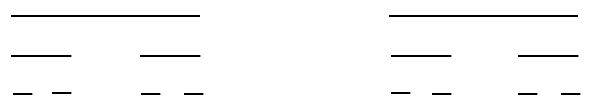
\includegraphics[width=0.75\textwidth]{image/CantorSet.jpg}
\vspace*{-0.3cm}
\caption{康托尔集的构造} \label{fig12}
\end{figure}

\noindent 令~$C = \smallcap^\infty \limits_{n=1} C_n$, 称为康托尔集\index{康托尔集}. 康托尔集具有以下性质:

\smallskip

(1) 康托尔集是闭的疏朗集(康托尔集无内点).

\smallskip

\begin{proof}
由闭集的性质易知康托尔集~$C$~是闭集. 为证~$C$~为疏朗集, 只需证明~$C^\circ = \emptyset$, 即任意~$C$~中的点都不是内点. 假设存在~$x \in C^\circ$, 则~$\exists~\varepsilon_0 > 0$, 使得~$(x-\varepsilon_0,\,x + \varepsilon_0) \subset C$. 取足够大的~$n_0$~使得~$1/3^{n_0} < \varepsilon_0$, 则~$(x-\varepsilon_0,\,x + \varepsilon_0)$~中必含有不属于~$C_{n_0}$~的点, 这与~$(x-\varepsilon_0,\,x + \varepsilon_0) \subset C = \smallcap\limits_{n=1}^\infty C_n$~矛盾.
\end{proof}

(2) 构造康托尔集从~$[0,\,1]$~中去掉的开区间长度之和为~$1$.

\smallskip

\begin{proof}
第~$n$~步, 去掉了~$2^{n-1}$~个长度为~$1/3^n$~的区间. 因此, 去掉的开区间长度之和为
\[
\sum^\infty _{n=1} \frac{2^{n-1}}{3^n} = \frac{1}{3}\sum^\infty _{n=1} \Big(\frac{2}{3}\Big)^{n-1} = 1
\]
\end{proof}

\smallskip

(3) 康托尔集是完全集(康托尔集每个点都是聚点).

\smallskip

\begin{proof}
设~$x \in C$, 则~$x \in C_n, \, n =1,\,2,\,\cdots$, 故对每个~$n \in \N$, $x$~属于长度为~~$1/3^n$~的闭区间
中的某一个, 记为~$F_n$. 于是, 对~$\forall~\varepsilon > 0$, 存在足够大的~$n_0$~使得~$1/3^{n_0} < \varepsilon$, 故~$F_{n_0} \subset U(x,\,\varepsilon)$. 又~$F_{n_0}$~的两个端点都属于~$C$, 故至少有一个端点不是~$x$, 记为~$x'$, 从而~$x' \in U(x,\,\varepsilon) \bigcap \big(C - \{x\}\big) \neq \emptyset$, 即~$x \in C'$.
\end{proof}

(4) $\overline{\overline{C}} = \overline{\overline{[0,\,1]}}$.

\smallskip

\begin{proof}
考虑~$[0,\,1]$~中的点用三进制小数表示. 去掉的开区间~$\big(1/3,\,2/3\big)$~
中的每个点~$x$~可表示为
\[
x = 0.1x_2x_3\cdots,\ \mbox{其中, } x_2,\,x_3,\,\cdots \in \{0,\,1,2\}
\]
区间端点~$1/3$~和~$2/3$~(属于~$C$)作特殊处理, 两种表示
\[
\frac{1}{3} = 0.100\cdots = 0.022\cdots, \quad \frac{2}{3} = 0.122\cdots = 0.200\cdots
\]
都采用后一种表示(不出现``1''). 去掉的开区间~$\big(1/9,\,2/9\big)$~
和~$\big(7/9,\,8/9\big)$~中
的点~$x$~可表示为
\[
x = 0.01x_3x_4\cdots \quad \mbox{~或~} \quad x = 0.21x_3x_4\cdots
\]
其中,  $x_3,\,x_4,\,\cdots \in \{0,\,1,2\}$. 区间端点~$1/9,\,2/9,\,7/9,\,8/9$~(属于~$C$)采用如下表示
\[
\frac{1}{9} = 0.0022\cdots, \quad \frac{2}{9} = 0.0200\cdots
\]
\[
\frac{7}{9} = 0.2022\cdots, \quad \frac{8}{9} = 0.2200\cdots
\]
依此类推, 去掉的开区间中的点必出现``1'', 而~$C$~则与所有不出现~``1''的小数一一对应, 即
\[
C \sim \big\{0.x_1x_2x_3\cdots: \: x_k \in \{0,\,2\}\big\}
\]
而
\[
\big\{0.x_1x_2x_3\cdots: \: x_k \in \{0,\,2\}\big\} \sim \big\{0.x_1x_2x_3\cdots: \: x_k \in \{0,\,1\}\big\}
\]
上式右端即为~$[0,\,1]$~的二进制小数表示, 故与~$[0,\,1]$~对等. 因此,
$\overline{\overline{C}} = \overline{\overline{[0,\,1]}}$.
\end{proof}

\begin{definition}
定义如下函数
\[
C(x)=\left\{\!\!
\begin{array}{cl}
0, & x = 0 \\[0.2cm]
\dfrac{2k-1}{2^n}, & x \in I_{n,k}  \\[0.2cm]
1, & x = 1
\end{array}
\right.
\]
其中, $I_{n,k}$($n=1,\,2,\,\cdots; \; k=1,\,\cdots, 2^{n-1}$)为康托尔集在构造过程中第~$n$~步挖去的
三分开区间, 该函数称为康托尔函数\index{康托尔函数}.
\end{definition}

康托尔函数~$C(x)$~是~$[0,\,1]$~上的单调递增的连续函数.

\newpage

\section*{附注~一}

\subsection*{实数的进制表示与转换}

下面介绍一下实数的~$p$~进制表示, $p \geqslant 2$~为整数. 首先回忆一下~$10$~进制表示
\[
256 = 2 \times 10^2 + 5 \times 10^1 + 6 \times 10^0
\]
\[
\pi = 3 \times 10^0 + 1 \times 10^{-1} + 4 \times 10^{-2} + \cdots
\]
\[
4.6799\cdots = 4.68
\]

类似地, 设~$x$~为一正实数, $p \geqslant 2$~为整数, 则~$x$~的~$p$~进制表示可以写成
\begin{eqnarray*}
x &=& b_m p^m + b_{m-1} p^{m-1} + \cdots + b_0 p^0 + a_1 p^{-1} + \cdots + a_n p^{-n} + \cdots \\
&=& \sum_{i=0} ^m b_i p^i + \sum_{j=1} ^\infty a_j p^j \\
&=& b_m b_{m-1} \cdots b_0.a_1 \cdots a_n \cdots
\end{eqnarray*}
其中, $b_i,\,a_j \in \{0,\,1,\,\cdots,\, p-1\}$. 若~$a_i$~从第~$i_0$~项之后都为~$p-1$, 而~$a_{i_0} \neq p-1$, 则把~$x$~表示为
\[
b_m b_{m-1} \cdots b_0.a_1 \cdots (a_{i_0}+1)
\]

上面的等式说明把~$x$~表示为一个正项级数, 其部分和~$S_{m+1+n}$~即为~$x$~的保留至第~$n$~位小数. 负实数~$y = - (-y)$, 则~$y$~的~$p$~进制表示即为正实数~$-y$~的~$p$~进制表示前面加负号. 因此, 每一个实数都可以
表示成~$p$~进制, 这也表明实数不同进制之间存在一一对应的关系.

$10$~进制转~$p$~进制算法:

\medskip

\begin{example}
$(14.267)_{10} = (~?~)_{3}$.
\end{example}

\begin{solution}
整数部分
\[
\left.
\begin{array}{l}
3~ | \! \underline{~14~~} \\[-0.2em]
~~3~ | \! \underline{~4~~} ~\cdots\cdots~ 2~ \quad b_0 \\[-0.2em]
~~\ 3~ | \! \underline{~1~} ~\cdots\cdots~ 1~ \quad b_1 \\[-0.2em]
~~~~~~~0~~\cdots\cdots~ 1~ \quad b_2
\end{array}
\right.
\quad \Longrightarrow \quad (14)_{10} = (112)_3
\]
小数部分
\[
\left.
\begin{array}{l}
~~0.267 \\[-0.3em]
\underline{\times ~~~~~3~} \\[-0.1em]
~~0.801 ~\cdots\cdots~ 0 ~\quad a_1 \\[-0.3em]
\underline{\times ~~~~~3~}  \\[-0.1em]
~~2.403 ~\cdots\cdots~ 2 ~\quad a_2 \\[-0.2em]
~~0.403 \\[-0.3em]
\underline{\times ~~~~~3~}  \\[-0.1em]
~~1.209 ~\cdots\cdots~ 1 ~\quad a_3 \\[-0.2em]
~~0.209 \\[-0.2em]
~~~~~\vdots ~~~~~~~~~~~~~~\vdots~~~~~\vdots
\end{array}
\right.
\quad \Longrightarrow \quad (0.256)_{10} = (0.021\cdots)_3
\]
故~$(14.267)_{10} = (112.021\cdots)_{3}$.
\end{solution}

$q$~进制转~$p$~进制算法: $q$~进制~$\rightarrow$~$10$~进制~~$\rightarrow$~$p$~进制.

\subsection*{集合悖论}

本章我们将集合定义为``具有确定内容或满足一定条件的事物的全体'', 这在历史上也曾被认为是一种满意的说法. 但在~20~世纪初, 英国逻辑学家罗素提出了下述悖论\footnote{悖论, 是指这样一个命题~$A$, 从~$A$~出发可以导出一个语句~$B$. 然而, 若假定~$B$~真, 则可推知~$B$~不真; 若假定~$B$~不真, 又推知~$B$~真. }
(也称为罗素悖论)
\begin{center}
``令~$X=\{E:\: E \in E\}$, 问集合~$X$~是否属于~$X$?''
\end{center}

该悖论给数学界带来了灾难性的后果! 它震撼了整个数学界乃至整个思想界, 从而促发了第三次数学危机.

\subsection*{集合论公理系统}

为了克服罗素悖论, 人们试图把集合论公理化, 用公理对集合加以限制.
第一个常用的公理系统是策梅洛和弗伦克尔等提出的~Z-F~集合论公理系统.
这个系统中只有一个非逻辑二元关系符号~``$\in$'', 非逻辑公理有: 外延公理、空集公理、无序对公理、并集公理、幂集公理、无穷公理、
分离公理模式、替换公理模式、正则公理, 再加上选择公理就构成~Z-F-C~系统.

利用公理可以定义出空集、序对、关系、函数等集合, 还可以给出序关系、良序关系、
序数、基数, 也可以给出自然数、整数、实数等概念. 集合论中有关集合的性质,
在公理集合论中都可以得到证明.\ 公理系统中还可以证明公理之间的相对和谐性和独立性,
例如, 柯恩于~1960~年创立公理集合论中的力迫法, 并用来证明~Z-F-C~系统与
连续统假设独立. 公理集合论发展很快, 马丁公理、苏斯林假设等新公理新方法已被广泛使用,
组合集合论、描述集合论、大基数、力迫法的研究已经渗透到数学的各个分支.

\subsection*{连续统假设}

关于无限集的基数, 我们知道最小的是可列集的基数~$\aleph_0$, 其次是实轴~$\R$~为代表的连续基数~$c$. 那么在~$\aleph_0$~和~$c$~之间是否还存在别的基数？这一问题曾耗费了康托尔本人不少的精力, 但并没有得出任何结论.

1900~年, 希尔伯特在巴黎数学家大会上提出了~23~个最重要的问题供~20~世纪的数学家们去研究, 这就是著名的``希尔伯特~23~个问题''. 其中列在首位的问题就是连续统假设

\begin{center}
``$\aleph_0$~与~$c$~之间不存在其他基数''
\end{center}

虽经后继者的许多努力, 也提出了若干等价的原则, 但还没有一个绝对的观念来说这一
猜测的真假. 不过在如今的~Z-F~集合论公理系统里, 哥德尔在~1940~年发表的文章中
证明了连续统假设的相容性(即连续统假设与~Z-F~集合论公理系统不矛盾). 而在~1963~年柯恩又证明了它的独立性(即连续统假设与~Z-F~集合论公理系统是相互独立的). 因此, 在目前最广泛采用的集合论公理系统中, 这一问题就算有了一个解答. 当然, 有的数学家认为: 应当有一个确定的集合理论出现, 使其中连续统假设是真或是假得到肯定回答.

\newpage

\begin{problemset}

\item 证明下列关于集合的关系式
\begin{enumerate}
\item[(1)] $A - (B-C) \subset (A-B) \cup C$.
\item[(2)] $(A-B)\cap (C-D) = (A \cap C)-(B \cup D)$.
\item[(3)] $A - (B - C) \subset (A - B) \cup C$. 问取~``=''~的充分必要条件是？
\item[(4)] 问~$A \cup (B-C) = (A \cup B) - C$~是否成立？
\end{enumerate}

\item 证明: $\{x : \: x>0\} = \smallcup\limits_{n=1}^\infty \big\{x: \: x > 1/n \big\}$.

\item 证明: $B - \limsup\limits_{n \to \infty} A_n = \liminf\limits_{n \to \infty} \big(B - A_n\big)$.

\item 设~$A_{2k-1} = \big(0,\, 1/k\big), \, A_{2k} = (0,\,k)$, $k=1,\,2,\,\cdots$, 求集列~$\{A_n\}$~的上限集和下限集.

\item 设当~$n$~为奇数时, $A_n = \big(0,\,1- 1/(n+2)\big)$; 当~$n$~为偶数时, $A_n = \big(1/n,\,1\big)$. 证明~$\lim\limits_{n \to \infty} A_n$~存在, 并求该极限.

\item 设~$f(x)$~为~$E$~上的实值函数, 则对任意的~$a \in \R$~有
\[
\big\{x \in E: \: f(x) > a \big\} = \medcup_{n=1}^\infty \Big\{ x \in E: \: f(x) > a+ \frac{1}{n} \Big\}
\]

\item 设~$\{f_n(x)\}$~为~$E$~上的实值函数列, 满足
\[
f_1(x) \leqslant f_2(x) \leqslant \cdots \leqslant f_n(x) \leqslant \cdots
\]
\[
\lim_{n \to \infty} f_n(x) = f(x)
\]
证明: 对任意~$a \in \R$, 都有
\[
\big\{ x \in E: \: f(x) > a \big\} = \medcup_{n =1}^\infty \big\{ x \in E: \: f_n(x) > a \big\}
\]

\item 设~$\{f_n(x)\}$~为~$E$~上收敛的实值函数列, 其极限函数记为~$f(x)$, 证明: 对~$\forall~a \in \R$~有
\[
\big\{x \in E: \: f(x) > a \big\} = \medcup_{k=1}^\infty \liminf_{n \to \infty} \Big\{x \in E: \: f_n(x) > a+\frac{1}{k} \Big\}
\]

\item 设~$X$~为全集, $A, \, A_\alpha \subset X, \, \alpha \in \mathnormal{\Gamma}$, 则
\begin{enumerate}
\item[(1)] $A = X$ $\Longleftrightarrow$ $\chi_A(x) = 1$;
\item[(2)] $A = \emptyset$ $\Longleftrightarrow$ $\chi_A(x) = 0$;
\item[(3)] $\chi_{\smallcup\limits_{\alpha \in \mathnormal{\Gamma}} A_\alpha} (x) = \max\limits_{\alpha \in \mathnormal{\Gamma}} \chi_{A_\alpha} (x)$;
\item[(4)] $\chi_{\smallcup\limits_{\alpha \in \mathnormal{\Gamma}} A_\alpha} (x) = \min\limits_{\alpha \in \mathnormal{\Gamma}} \chi_{A_\alpha} (x)$.
\end{enumerate}

\item 设~$\{A_n\}$~为集列, 证明\footnote{该结论表明: 集列的极限存在等价于函数列~$\{\chi_{\tiny{A_n}}(x)\}$~的极限存在. }
\[
\chi_{\limsup\limits_{n \to \infty} A_n}(x) = \limsup_{n \to \infty} \chi_{A_n}(x), \, \quad \chi_{\liminf\limits_{n \to \infty} A_n}(x) = \liminf_{n \to \infty} \chi_{A_n}(x)
\]

\item 证明: 单位圆周与整个实数轴对等.

\item 设~$\{A_n\}, \, \{B_n\}$~分别为两两互不相交的集列, 若~$A_n \sim B_n, \, n=1,\,2,\,\cdots$, 则对任意的~$N$~(有限或为~$+\infty$), 都有~$\smallcup\limits_{n=1}^N A_n \sim \smallcup\limits_{n=1}^N B_n$.

\item 设~$A_1 \smallcap A_2 = \emptyset, \, B_1 \smallcap B_2 = \emptyset$, 又~$\varphi_1:\:A_1 \rightarrow B_1,\, \varphi_2:\: A_2 \rightarrow B_2$~为两个一一映射, 若~$A_1 \subset A_2, \, B_1 \subset B_2$, 问是否存在~$A_2-A_1$~到~$B_2-B_1$~上的一一映射?

\item 用另一种方法证明定理~\ref{thm1.3.7}. (提示: 构造一一映射)

\item 证明: 有理数多项式全体构成的集合是可列集.

\item 证明: 平面上坐标为有理数的点组成的集合为可列集.

\item 设~$A$~为平面上以有理数点为中心, 以有理数为半径的圆的全体构成的集合, 则~$A$~为可列集.

\item 设~$B$~为自然数列的全体构成的集合, 问~$B$~与~$\N$~对等吗?

\item 设实轴上所有闭区间的全体构成的集合为~$E$, 则~$\overline{\overline{E}} = \aleph$.

\item 用~$\R^\infty = \big\{\{x_1, \, x_2, \, \cdots\}: \: x_i \in \R \big\}$~表示实数列的全体, 证明: $\overline{\overline{\R^\infty}} = \aleph$.

\item 用~$C[0,\,1]$~表示~$[0,\,1]$~上实值连续函数的全体,
      则~$\overline{\overline{C[0,\,1]}} = \aleph$.

\item 若~$\overline{\overline{\smallcup\limits_{n=1}^\infty A_n}} = \aleph$, 则必存在~$n_0$~使得~$\overline{\overline{A_{n_0}}} = \aleph$.

\item 证明: 设~$f(x)$~为~$(a,\,b)$~上的凸函数, 即对任意的~$x_1,\,x_2 \in (a,\,b)$~以及~$\lambda \in (0,\,1)$, 都有
\[
f\big(\lambda x_1+(1-\lambda)x_2 \big) \leqslant \lambda f(x_1) + (1- \lambda) f(x_2)
\]
则~$f(x)$~在除了一个至多可列集外的点上都是可微的.

\item 举例给出具有下列性质的点集:
\begin{enumerate}
  \item[(1)] $A_1$~只有一个极限点, 且极限点不属于~$A_1$;
  \item[(2)] $A_2$~有可列个极限点, 且极限点不属于~$A_2$;
  \item[(3)] 有边界点, 但边界点不属于该集合的平面点集;
  \item[(4)] 极限点一部分在集合中, 另一部分不在集合中, 甚至极限点比集合本身的点还要多.
\end{enumerate}

\item 设~$X = \R^2$~($xOy$~平面)为全集.

\begin{enumerate}
\item[(1)] $A = \{ (x,\,y): \: x^2 + y^2 < 1\}$, 求~$A',\, A^\circ,\,\overline{A}$;
\item[(2)] 设~$B = \{(x,\,y):\: x \in \R, \, y=f(x)\}$, 其中
\[
f(x) = \left\{ \!\!
\begin{array}{cl}
\sin \dfrac{1}{x}, & x \neq 0 \\[0.2cm]
0, & x=0
\end{array}
\right.
\]
求~$B',\,B^\circ$.
\end{enumerate}

\item 设~$A \subset \R^n$~为闭集, $B \subset \R^n$~为开集, 且~$A \subset B$, 则存在~$d > 0$~使得~$\smallcup\limits_{x \in A} U(x,\,d) \subset B$.

\item 设~$E \subset \R$~为可数集, 证明存在一点~$a \in \R$~使得~$E \cap \big(E + \{a\}\big) = \emptyset$.

\item 证明: 无理数的全体不能表示为可数个闭集的并.

\item 设~$f(x)$~为~$\R$~上的实值函数, 若~$f$~把任一开集映为开集,
      问~$f(x)$~是否连续? 又连续映射是否一定映开集为开集?

\item 设~$f(x)$~为~$\R$~上的连续函数, 证明对任意的~$a \in \R$:

\noindent (1) $\{x \in \R: \: f(x) > a\}$~与~$\{x \in \R: \: f(x) < a\}$~都是开集;

\noindent (2) $\{x \in \R: \: f(x) \geqslant a\}$~与~$\{x \in \R: \: f(x) \leqslant a\}$~都是闭集.

\item 设~$E$~为孤立点集, 问~$E$~上的任一函数是否连续? 是否一致连续?

\item 是否存在~$[0,\,1]$~上的函数, 满足它在每个有理数点不连续, 而在每个无理数点都连续?

\item 是否存在~$[0,\,1]$~上的函数, 满足它在每个有理数点都连续, 而在每个无理数点都不连续?
\end{problemset}
